\documentclass[12pt,titlepage,oneside]{book}

\usepackage[T1]{fontenc} % modern encoding
% Comment out the next three lines of LaTeX if you wish to use Computer Modern fonts
%   (this is the default for LaTeX)
% Make sure that your TeX installation can produce good pdf with these fonts.
% The following three lines are a good alternative if you don't use much mathematics
\usepackage{mathptmx}  % uses Times for text and mathematics
\usepackage[scaled]{helvet} %  helvetica for sanserif, scaled 95% by default
\usepackage{courier}  % courier for typewriter font, pretty ugly but available
% otherwise the stix package offers more options and symbols
% \usepackage{stix}  % uses Times for text and a range of fonts for mathematics
% End of choices for fonts
\usepackage{graphicx}  % standard package for importing graphics files
%\usepackage{cite}  % improves format of numerical citations, such as [1-3]
\usepackage[top=2cm,bottom=2cm,left=4.0cm,right=2cm]{geometry}
% These margins are the university guidelines
\usepackage[onehalfspacing]{setspace}  % gives one-and-a-half line spacing

\usepackage{nomencl}
\makenomenclature

% Added packages
\usepackage[parfill]{parskip} % gives paragraph separation

% graphing and diagrams
\usepackage{siunitx}
\sisetup{per=slash, load=abbr}
\usepackage{tikz}
\usepackage{pgfplots}
\usepackage{xcolor}

\pgfplotsset{compat=1.15
%, width)\textwidth
}
\usepackage{textcomp}
\usetikzlibrary{shapes,arrows,circuits.ee.IEC}

\usepackage{subcaption}

\usepackage[sortcites, sorting=none, maxbibnames=99]{biblatex}
\DeclareNameAlias{default}{family-given}
%\bibliographystyle{acm.bst}
\bibliography{bibliography.bib}

%\bibliographystyle{plain}
%\bibliographystyle{unsrt} % orders based on order of citation


\usepackage[english]{babel}
\addto\captionsenglish{\renewcommand\chaptername{Section}}  % changing "chapter" to "section" at the top of each page

% formatting chapter headings
\usepackage[T1]{fontenc}
\usepackage{titlesec, blindtext, color}
\definecolor{gray75}{gray}{0.5}
\newcommand{\hsp}{\hspace{6pt}}
\titleformat{\chapter}[hang]{\Huge\bfseries}{\thechapter\hsp\textcolor{gray75}{| }\hsp}{0pt}{\Huge\bfseries}

\usepackage{listings} % for source code


\begin{document}
\begin{titlepage}
\centering
\vspace*{3cm}  % Need the * or the space is swallowed at the top of the page
\bfseries\Large
Using an FPGA to Enhance Functional Safety in an Automatic Transfer Switch\\
% FPSoC? Field Programmable System-on-Chip (ADC, memory etc.)


\vspace{3cm}
\normalfont\large
Andrew Smith 2198699s\\
MEng Electronic and Software Engineering\\
\vspace{2cm}
ENG5041P: Individual Project 5\\

\vspace{2cm}
Primary Academic Supervisor: Professor Scott Roy\\
Secondary Academic Supervisor: Professor Edward Wasige\\
Industrial Supervisor: Julien Guilhemsang PhD\\
\vspace{1cm}
\includegraphics[scale=0.125]{images/GlaLogo.pdf}
\\
\vspace{1cm}
% Insert month and year of date deposited with library for final version
2019-20
\end{titlepage}
\frontmatter  % Turn off chapter numbering, use roman page numbers
\chapter{Abstract}
Safety-critical applications require reliable power supplies. Due to recent trends in the adoption of renewable power sources, being able to switch between power supplies is necessary to keep safety-critical systems, such as hospitals and data-centres, online. The overall aim of this project was to investigate automatic transfer switch (ATS) technology to propose an FPGA-based solution drawing on the relevant safety standards, representing a new approach for a large power supply manufacturer. A prototype was developed in order to evaluate the differences between an existing microcontroller based system and the FPGA-based alternative designed and implemented by this project. The prototype implemented the safety function of the device: controlling the motor which performs the transfer. The V-model for the design and verification of ASICs was applied to the FPGA development process. The FPGA-based system acted as a proof of concept, providing substance for an evaluation of FPGA adoption in ATS motor control. The FPGA-based system successfully replicated the motor control behaviour of the ATS, improving the response time and accuracy of the regulation process as well as increasing the PWM resolution. Through following the published safety standards and by verifying the solution, the foundations for ATS functional safety have been established by this project. The prototype will lead to a new, safer product which will enhance the existing ATS product line.
\chapter{Acknowledgements}


I would like to thank Professor Scott Roy and Professor Edward Wasige at the University of Glasgow for supervising this project.

I would also like to thank Julien Guilhemsang and J\'er\^ome Viriot at Socomec for their continued support throughout the placement. 

Additionally I would like to thank the development team at Socomec for 
%and for 
being patient with me as I familiarised myself with the French language.

%\include{declaration}

\renewcommand{\contentsname}{Report Contents} % change the contents page title
\cleardoublepage
\tableofcontents
\listoftables
\listoffigures



\renewcommand{\nomname}{Abbreviations}

\mbox{}
\nomenclature{$FPGA$}{Field Programmable Gate Array}
%\nomenclature{$FPSoC$}{Field Programmable System on Chip}
\nomenclature{$PLD$}{Programmable Logic Device}
\nomenclature{$OSVVM$}{Open Source VHDL Verification Methodology}
\nomenclature{$UVVM$}{Universal VHDL Verification Methodology}
\nomenclature{$SIL$}{Safety Integrity Level}
\nomenclature{$E/E/PE$}{Electrical/Electronic/Programmable Electronic}
\nomenclature{$ATS$}{Automatic Transfer Switch}
\nomenclature{$ATyS$}{Socomec Brand ATS}
\nomenclature{$IGBT$}{Insulated-Gate Bipolar Transistor}
%\nomenclature{$HDL$}{Hardware Description Language}
\nomenclature{$PWM$}{Pulse Width Modulation}
\nomenclature{$PCB$}{Printed Circuit Board}
\nomenclature{$UUT$}{Unit Under Test}


\printnomenclature

\mainmatter % Turn on chapter numbering, reset page numbers, use arabic

\chapter{Introduction}
\label{introduction}

% What is the problem: necessity of supplying consistent sources in nuclear and hospitals etc 
In a safety-critical application, the failure or malfunctioning of equipment can result in loss of life, serious injury or damage to the environment\cite{HayekSafety, Borcsok}. For example, the failure of hospital equipment can be fatal. In these environments, the effects of power cuts can be devastating\cite{azeem, onipede}. The reliability of the supply of power to these systems is essential especially with recent trends towards renewable sources for which a consistent supply to applications cannot be guaranteed\cite{liserre, onipede}.

% what is the solution to this problem
An Automatic Transfer Switch (ATS) is a device that ensures a reliable power source is available to critical loads in a system\cite{azeem}. This involves monitoring two separate sources and switching between them if necessary. ATS devices have been adopted in a number of environments, including nuclear and medical, to ensure that safety-critical operations can be performed. Consequently, in the development of ATS systems, functional safety and verification are imperative to guarantee that the critical loads are transferred appropriately.

This report describes the design, implementation and verification of a new ATS processor for use in safety-critical applications. All work described in this report was carried out as part of the MEng project for the Socomec Group. Socomec was established in 1922 in Alsace, France, specialising in the control and security of electrical supplies. Currently, there are 28 subsidiaries around the world and have a turnover of 537 million euros. This project was conducted in the global headquarters in Benfeld, France.

%Additional measures must be taken and safety-related standards must be followed to ensure that the system operates correctly. 

\section{The Socomec ATyS}
% what is the current design
The Socomec Group product range includes a microcontroller-based ATS device. An example ATyS, the commercial name given to Socomec ATS devices, can be seen in Figure \ref{AtysDevice}. The Socomec range can handle a range of power supplies from 125A to 3200A\cite{socomec_atys_range}. It is implemented using two control boards: the first is used to monitor the supplies and determine whether it is necessary to perform a transfer, the other board is responsible for performing the physical switch between the supplies by driving a universal motor. Each of these control boards use a microcontroller as the processor.
% atys connection / configuration
An example network configuration of the ATyS, where it controls the connection of the circuit between a mains power supply and a back-up generator, is shown in Figure \ref{AtysConfig}. Several configurations are possible for the ATyS but the principle remains the same: ensure a reliable supply of power.

\begin{figure}[h]
\centering
\includegraphics[width=0.6\textwidth]{images/ATySDevice.jpg}
\caption{The Socomec Automatic Transfer Switch (ATyS)\cite{socomec_atys}}
\label{AtysDevice}
\end{figure}


\begin{figure}[h]
\centering
\includegraphics[width=0.7\textwidth]{images/AtysConfig.pdf}
\caption{Example ATyS configuration controlling a load connection between mains (green) and a back-up generator (pink)\cite{socomec_atys_network}}
\label{AtysConfig}
\end{figure}


\section{Project Aims}

% what change is being made to the design and why
The project, outlined in this report, involves replacing the micro-controller processor in the ATyS motor control board with a Field Programmable Gate Array (FPGA). The primary motivation for this change is to enhance the functional safety of the ATyS system where functional safety is defined as "ensuring the correct behaviour of a system and detecting or correcting when the behaviour is not as expected"\cite{Jeppesen, IECfunctionalsafety}. 
% nature of the project (proof of concept, investigation into safety requirements (e.g. verification), prototype (design) with focus on the safety function of the device)
The overall aim of the project is to investigate the advantages of an FPGA-based solution with a focus on the functional safety of the device. In order to do this, the project had the following objectives:
\begin{itemize}
  \item Conduct a literature review to discover where FPGAs have been used in similar systems
  \item Analyse the related safety standards and determine how they could be applied to an FPGA-based system
  \item Design an FPGA-based alternative solution from the existing micro-controller specification
  \item Develop VHDL code to implement the design using processes and tools recommended by the safety standards  
  \item Verify the design in accordance with the recommendations of the safety standards
  \item Physically prototype the FPGA-based solution and compare the response with the original solution
\end{itemize}

%This will involve the development of a PCB with an FPGA processor onto which a VHDL design will be synthesised.   

% comparison with the existing solution: how will the project be evaluated

\section{Report Structure}
% how the report will be structured
This report will begin by reviewing literature in areas relevant to this project. As part of this, the theory behind the chosen methodologies for this project is presented and similar projects are discussed. Following this, the design and implementation of the prototype FPGA-based system are presented in Section \ref{design}. The verification of this design is then presented in Section \ref{verification}. The behavioural results of the prototype are discussed and compared against the existing solution in Section \ref{results}. The results of the project are evaluated in Section \ref{evaluation} against the initial aims and objectives outlined in this section and suggestions for further work are presented. Finally, the conclusions drawn from the project are summarised.

\chapter{Literature Review}
\label{litreview}

This section presents the existing literature that underpins the central themes of the project. The relevant safety standards that need to be followed for the project are introduced first. The application of these standards to FPGA-based projects is then reviewed. Examples of the application of FPGAs in safety-critical and industrial switching applications are then explored. To highlight the context of FPGAs as a possible solution, a comparison is made between FPGAs, microcontrollers and ASICs regarding their use in these application areas. 
%Additionally, features of FPGAs which make them suitable for safety-critical designs are discussed through previous, similar industrial switching projects. 
Finally, the design methodology which has been adopted for the project, and that is recommended by the standards, is presented and discussed. Verification methodologies are also introduced in this section.

\section{Safety-Critical Systems}
A safety-critical system is defined as "a system whose failure or malfunction may result in death or serious injury to people, damage to equipment or environmental harm"\cite{Bernardeschi}. In the design of these systems, safety standards must be followed\cite{Bernardeschi, HayekSRAM, HayekSafety}.

\subsection{Electronic Safety Standards}
The IEC 61508 set of standards covers the use of electrical, electronic and programmable electronic devices in safety-critical systems\cite{IEC61508}. Within these standards, Safety Integrity Levels (SIL) are defined. They represent the functional safety level of a device application. The SIL framework has two main aims in providing functional safety: the prevention of systematic errors through thorough design processes and the detection and control of any errors in the device\cite{IEC61508}. They also provide a standardised methodology for claiming the safety integrity for an electronic device\cite{Redmill, Borcsok}. 

\subsection{FPGAs in Safety Standards}
  
There is an absence of safety-related standards for the application of programmable logic devices (PLDs) such as FPGAs\cite{DaSilva,Conmy,Bernardeschi}. Without specific reference in safety standards, it can often be unclear which standards should apply to FPGA-based systems\cite{DaSilva,Conmy,Borcsok}. This has resulted in the adoption of standards and techniques for related, general technologies such as for electrical, electronic and programmable electronic devices\cite{Bernardeschi}. In the absence of specific PLD standards, certain aspects specific to PLD/FPGA devices are not fully covered by the standards\cite{DaSilva}. These relate to the inconsistency of the classification of FPGAs which contain aspects similar to both hardware and software designs\cite{Conmy,DaSilva}. 
This can make it difficult to verify the safety of these systems\cite{DaSilva,Conmy}. % examples
However, by separating the analysis of the design code and the target device, it is possible to assess the safety of FPGA systems\cite{HayekSRAM, Borcsok}. In this way, FPGAs can be treated as ASICs in regards to functional safety\cite{HayekSRAM, HayekSafety, Bernardeschi}.
  
\section{Use of FPGAs in Safety-critical Systems}

The FPGA market has been growing and expanding into new application areas\cite{Foster} and safety-critical applications, in particular, have seen increased adoption of FPGAs\cite{Foster,DaSilva,Conmy,HayekSafety,HayekSRAM,Bernardeschi,Cilardo, SalewskiExploring}. Safety-critical application domains which have already adopted FPGA technology include aerospace, industrial control and military\cite{Foster,Bernardeschi}. Rodr{\'\i}guez-Andina states that ``Digital control of power systems is one of the most interesting current research topics in industrial electronics''\cite{Rodriguez} and FPGAs are commonly applied to these fields\cite{MonmassonDesign, Gomes, Dubey, deCastro}. 

The time which electronic components remain available on the market has been reducing\cite{Guzman-Miranda}. The rapid development of new technologies requires components to be regularly updated in order to compete in the market\cite{Sandborn}. This poses a major problem for safety-critical systems which, due to their intense verification process, are required to stay operational for extended periods\cite{Guzman-Miranda, SalewskiFaultHandling}. When system components which implement the safety function become unavailable, the lifetime of the entire system may be cut short\cite{Guzman-Miranda}. 

There are a number of classic solutions to this problem including stockpiling components, reverse engineering the unavailable components, requesting manufacturers to fabricate more of the required components, or redesigning affected areas of the system\cite{Guzman-Miranda}. FPGAs provide an elegant solution to this problem, being able to implement obsolete digital components, for example, microprocessors, to ensure that they are always available for use\cite{Guzman-Miranda, Malinowski}. Especially with recent advancements in the technology, FPGAs are able to model more complex digital components and there is an existing market for such Intellectual Property\cite{Guzman-Miranda}.

\subsection{FPGAs in Industrial Control Projects}

In industrial control and safety-critical applications, there is a demand for lower cost and an increased expectation of performance\cite{MonmassonFPGADesignMethodology, SalewskiFaultHandling}. 
%Monmasson et al. present a number of industrial switching projects where FPGAs have been adopted including soft switching, motion control and induction machine drives\cite{MonmassonFPGADesignMethodology}.
FPGAs allow for the control functions to be implemented in hardware, giving the possibility of higher performance motor control\cite{jabeen}. The increase in performance means that FPGAs are now fast enough to ensure that processing speed is no longer the bottleneck in IGBT driving which can be applied to motor control\cite{MonmassonDesign}. Motor control applications also demand deterministic timings which FPGAs can provide\cite{Dubey, al-mahmood}. FPGAs have been specially adapted to these applications with the addition of functional units such as PWM generators and hardware timers\cite{deCastro}.

%FPGAs allow for rapid prototyping\cite{Dubey}.



\section{FPGA Features}

There are a number of benefits that FPGAs have over other embedded processors which make them appealing to designers. By performing parallel operations, FPGAs can offer enhanced performance\cite{Dubey,Foster,Al-Dhaher,Conmy,MonmassonFPGABasedControllers,MonmassonFPGADesignMethodology, deCastro} and can reduce calculation time and latency\cite{Rodriguez,Naouar,MonmassonFPGADesignMethodology}. FPGAs can also monitor multiple inputs and control multiple outputs concurrently and continuously\cite{SalewskiSystematic, deCastro, Zhang}. 
Since FPGAs operate concurrently, additional diagnostics can be added without impairing the performance of the system\cite{Dubey}. Additionally, diagnostic monitors can run continuously\cite{Dubey}.

Modern FPGAs, with dedicated resources, also have enhanced capabilities for interfacing with the analogue world compared to other embedded processors\cite{Rodriguez}. This means that they can perform like analogue components with minimal delays\cite{Aime} while providing additional benefits such as reduced noise and ease of control\cite{Naouar}. These benefits are desirable for the development of real-time systems.

%Although each of the devices can be used to implement the same system, differences in the design

FPGAs provide flexibility allowing systems to be redesigned at any stage\cite{Al-Dhaher}, for example, to respond to changes in the requirements\cite{Bernardeschi}. FPGAs also allows for features to be added to the system later in the design, such as monitors and diagnostics\cite{Jeppesen,MonmassonFPGABasedControllers}. This flexibility also adds a degree of design freedom, when compared to microcontrollers, allowing a variety of dedicated hardware architectures to be considered for the application\cite{Naouar, Idkhajine, Zhang}. 

\subsection{Microcontroller Comparison}

FPGAs, implemented in hardware description languages (HDLs), are synthesised as electronic components\cite{SalewskiSystematic}. This means that functional and timing behaviour is deterministic and predictable\cite{jabeen, wells}. As a result, the verification possibilities of these devices are enhanced\cite{HayekSafety, SalewskiExploring, SalewskiFaultHandling} with respect to microcontroller solutions developed in sequential programming languages such as C. The interrupt-driven behaviour and the use of caching mechanisms, adopted by microcontroller designs, means that it is difficult to accurately model and verify these systems\cite{wells, SalewskiExploring, SalewskiFaultHandling}. The differences between FPGAs and microcontrollers for use in safety-critical and real-time systems, due to this difference in behaviour, are summarised in Table \ref{safety-table}.

\begin{table}[t]
\centering
%\begin{tabular}{ |p{4cm}||p{4.5cm}|p{4.5cm}|  }
\begin{tabular}{ |p{0.2\textwidth}|p{0.35\textwidth}|p{0.35\textwidth}| }
 \hline
 \multicolumn{3}{|c|}{FPGA vs Microcontroller Real-time Safety Comparison} \\
 \hline
 Property & FPGA & Microcontroller \\
 \hline
 \hline
 Timing Behaviour & Deterministic timings: synthesised electronics with predictable timing behaviour that can be accurately simulated\cite{SalewskiExploring, jabeen, Dubey, tahoori, al-mahmood}  & Non-deterministic timings: Adoption of caching mechanisms and interrupts results in unpredictable timings\cite{SalewskiExploring, wells}   \\
 \hline
 Input Acquisition Model & Continuous monitoring: inputs are continuously monitored allowing the system to respond to events in realtime\cite{SalewskiExploring} & Time-slicing: inputs are monitored on a polling or interrupt-based system which introduces latency\cite{SalewskiExploring} \\

 \hline
 Operating Mode & Real parallelism: multiple calculation streams can be performed concurrently\cite{SalewskiExploring, Gomes, MonmassonDesign, NaouarSliding, SalewskiSystematic, Zhang, Al-Dhaher} & Simulation of parallel: sequential single-core processors can only handle one task at a time\cite{SalewskiExploring, Al-Dhaher}\\
 \hline
 Processing Speed & Quasi-analogue: adoption of optimised architectures reduces response times to quasi-analogue levels\cite{MonmassonFPGADesignMethodology, Idkhajine, Zhang} & Fast: micro-controllers can sometimes struggle in high demand environments or with complex calculations\cite{Zhang} \\
 \hline
 Application of Diagnostics & Parallel diagnostics: can run in parallel with the system operation without affecting performance\cite{Jeppesen} & Interrupt-based: diagnostics require processing to be taken away from the main system or be performed off-chip\cite{SalewskiExploring, Al-Dhaher} \\
 \hline
 Design Language &  Technology independent: HDL designs are independent of the hardware and so a different FPGA device can be used with minimal effort\cite{SalewskiExploring, SalewskiSystematic, Dubey, Zhang, deCastro, Acero} & Technology dependant: microcontroller firmware is often hardware-dependent making it more prone to obsolescence\cite{SalewskiExploring, SalewskiSystematic}   \\
 \hline
\end{tabular}

\caption{Comparison between FPGAs and micro-controllers for use in real-time safety-critical systems}
\label{safety-table}
\end {table}


\subsection{ASIC Comparison}

FPGA-based projects have been found to have a shorter time-to-market and lower non-recurring engineering costs than in ASIC development\cite{Foster,DaSilva,Bernardeschi, Borcsok, baines}. This has been accredited to FPGA re-programmability meaning that expensive silicon respins, which occur during ASIC development, are not necessary\cite{Bernardeschi, Borcsok}. The balance of costs can depend on a number of factors including package costs, area costs and development costs which all vary depending on the application\cite{kuon, baines}. FPGAs can be up to 100 times more expensive per-unit\cite{baines}. On the other hand, ASIC designs, depending on the fabrication and technology, can cost over \$1 million per spin\cite{zahiri}.
The reduced time-to-market means that FPGAs are often more cost-effective for low volume production\cite{Foster,Bernardeschi}. This has made FPGAs more popular for a variety of applications\cite{DaSilva, Dubey}. However, this re-programmability can encourage a reduced verification cycle and Foster finds that the reduced design life-cycle of FPGAs means that there is usually a higher number of bugs found in production compared to ASIC systems\cite{Foster}. The use of ASICs was not considered for this project due to the high up-front costs of ASIC prototyping.


\subsection{FPGA Verification}

As FPGA technology advances, the verification overhead increases\cite{DaSilva, Drechsler}. There is an increasing need for efficient verification of the functionality of these systems\cite{Foster,Rodriguez}. Modern FPGAs often resemble System-on-Chip (SoC) devices which are commonly referred to as FPSoCs\cite{Rodriguez,Naouar,MonmassonFPGAsIndustrialControlApplications,Bernardeschi}. With multiple functionalities and interfaces, verification becomes more of a challenge\cite{Foster}.

In terms of design safety and verification, FPGAs offer enhanced possibilities\cite{SalewskiFaultHandling}. Only the synthesised electronics must be verified whereas in microcontrollers it can be necessary to verify the software, hardware and the operating system\cite{SalewskiFaultHandling}. In order to achieve verification in FPGA designs, simulation of individual modules is required alongside the verification of the interactions between modules\cite{SalewskiSystematic}. System components which control the safety function should have 100\% coverage\cite{Ceesay-Seitz}. Simulation can be performed at each level of the design\cite{SalewskiSystematic} and it remains the dominant form of verification for HDL designs\cite{SalewskiSystematic, Yun}. Accurate timings can be modelled once the place and route are known\cite{SalewskiSystematic}.


\section{V-Model Development}

\begin{figure}[h]
\centering
%\includegraphics[width=0.8\textwidth]{images/Vmodel.pdf}
\includegraphics[width=\textwidth]{images/V-model.PNG}
\caption{The V-model for ASIC development adopted for design and verification in this project\cite{IEC61508}}
\label{V-model}
\end{figure}

Adoption of the V-model, see Figure \ref{V-model}, for ASIC and FPGA designs is recommended by Lattice for safety-related development\cite{LatticeSafety} as well as in the safety standards \cite{Borcsok, IEC61508, HayekSRAM, HayekSafety, Bernardeschi}. The model focuses on the verification and validation of the design at each design phase\cite{Borcsok}. For each design phase, there is a corresponding verification activity\cite{Ceesay-Seitz,Borcsok}. It incorporates methodologies from software development into the ASIC design process\cite{HayekSRAM}. As well as acting as an overall model for project development, the V-model can be traversed for subsystems and modules within the design\cite{Ceesay-Seitz}. HDLs support the adoption of the V-model as they allow for the behaviour and performance to be verified at each development phase of the project\cite{Dubey}.

\subsection{VHDL Verification Methodologies}

In order to tackle the increasing verification effort of FPGA designs, verification methodologies have emerged\cite{Foster}. There are a number of verification methodologies applicable to FPGAs and VHDL development. Verification is a large component of the design life-cycle. % find sources for this
Tallaksen finds that verification accounts for 50\% of the development effort for FPGA-based system\cite{Tallaksen}. It is a crucial activity which produces a valuable resource: automated and comprehensive test-suites provide a safety-blanket to ensure that any errors in the design are flagged\cite{janzen}.
%\subsection{Universal VHDL Verification Methodology}
One methodology, which is rapidly growing in popularity, is the Universal VHDL Verification Methodology (UVVM)\cite{Foster, Tallaksen}. The UVVM framework claims to provide overview, modifiability, debuggability and reusability to unstructured test-benches\cite{Tallaksen}.
%\subsection{Open Source VHDL Verification Methodology}
OSVVM (Open Source VHDL Verification Methodology) and UVVM have seen a considerable adoption for verification in FPGA-based design projects; in 2018 this was found to be 15\% and 10\% respectively\cite{Foster,Tallaksen}.

\section{Literature Review Conclusion} % should this be labelled? 

% safety standards being followed
FPGAs have seen considerable adoption in safety-critical and motor control. The relevant safety standards for the project are the IEC 61508 standards related to electronics development in safety-critical applications. Although there is no direct mention of FPGAs in this particular standard, FPGAs can be considered as ASICs throughout the development phases. 
The primary advantages of using FPGAs for safety-critical systems is having the ability to accurately model and verify timings and behaviour.
% increased verification effort -> verification methodologies -> functional safety now achievable
Advancements in FPGA technology have resulted in more complicated designs with multiple interfaces. This has introduced a significant verification requirement meaning that classic test-benches are no longer viable for complete verification. Verification methodologies, which have recently emerged, allow for the functional safety of FPGA systems to be achieved and proven. FPGAs also provide an elegant solution to component obsolescence, for which safety-critical systems are particularly vulnerable. 

% lack of coverage means the adoption of asic and software standards?
%Despite the increased adoption of FPGAs in safety-critical systems, there is a lack of FPGA-specific safety standards. This has resulted in the adoption of general standards and standards for related technologies which often fail to cover considerations specific to FPGAs.


% adoption of the v-model throughout the project 
The V-model, which is recommended for the standards, will be followed throughout the development of this project. It also forms the structure of this report. The following two sections traverse the V-model, discussing the high-level processes within the project. The design section, Section \ref{design}, discusses each of the activities on the left side of the V-model. In the verification section, Section \ref{verification}, the corresponding verification activities for each of the design phases are described. These are the activities on the right side of the V-model.




\chapter{Design and Implementation}
\label{design}

This section presents the design of the FPGA-based control board prototype. The design followed the top-down design stages of the V-model shown in Figure \ref{V-model}. This section follows the design flow by first discussing the requirements for the system and how they were identified. This includes the identification of the subset of requirements necessary to implement the safety function of the device. This is followed by a presentation of the architecture that was derived from these requirements. The design and implementation of the modules which form the architecture is then presented. The physical prototype, created as part of this project, is then discussed.

\section{V-Model Design Process}

%The V-model is an iterative methodology which promotes...

The design stages outlined in the V-model follow a top-down methodology. The methodology starts with the definition of the system and safety requirements.
From these requirements, an architecture is derived.
The behaviour of this architecture must then be modelled. 
Modules which form the architecture can then be designed.
The final stage of design, following the V-model, is the synthesis, placement and routing of the design. This stage involves the application of constraints to the synthesis environment as well as the mapping of the design.
Each of these activities are described in the following sections.


%The major focus of the V-model is on the verification of the design on every level. In order to achieve this, the system must be designed for testability. For example, on a module level, modules should be well contained, simple and have well-defined functionality. The reuse of modules also reduces the verification effort. 


\section{Prototype System Requirements}

An ATyS specification document was created by Socomec as part of a previous iteration of the device. 
% original ATyS requirements
This existing specification of the microcontroller-based system represents a full set of the requirements for the ATyS motor control. The motor control process has a number of operating modes and possible conditions. This includes the option to change the load motor as well as the command interface. For example, the commands can come from a customer input or from the source detection board of the ATyS. 


%\subsection{Prototype Scope and Safety Requirements}

For this prototype, the requirements which are necessary for performing the motor control were identified and this became the specification for the prototype.
Only safety features should be considered with respect to the functional safety of the device\cite{HayekSRAM}.
% requirements specification process - move this process to the safety requirements section?
The comprehensive microcontroller specification was used to derive the subset of requirements to be implemented as a prototype. The motor control process was identified as the safety function and so this was the central focus for the prototype design. It is the core behaviour of the device and performs the essential behaviour of changing the connection from one source to another. External PCB requirements are outside of the scope of this project. Only the motor control requirements that relate to the processor and its interfaces were considered for this design. The requirements for the prototype are outlined in Table \ref{requirements-table}.


%\subsection{Motor Control Process}

The overall process of motor control involves moving from the current position to a desired position and stopping when the position is reached. Several stages, which need to be performed in order to complete this process, are outlined in the existing specification. 
%The process begins with the driving of the required Thyristor and IGBT opposite pair (see Figure \ref{motor_control_circuit}). After this, a minimum PWM value is provided to the IGBTs. This value is increased until it reaches the maximum value and then the PWM duty-cycle is regulated based on the motor current. If the position is reached within five seconds, the motor is stopped. However; if the desired position is not reached within five seconds, the cycle is repeated and if still not successful after a further five seconds, the device is put into an error state and a relay is driven.
%\subsection{Requirements for Performing Motor Control}
% the requirements of this project 
The external interfacing requirements of the motor control process can be broken down into three sections. The first of which is the command input. This uses a simple command which is input to the device by activating a number of pins. 
The second requirement is the constant detection of the position. This is done using a series of pushbuttons, the state of which determine the physical position of the motor. 
The final required interface of the motor control safety function is the control of the motor.  
There are also internal requirements for the processing of these inputs and outputs. 
PWM regulation allows for accurate motor control. The regulation scheme is to use the motor current value to adjust the PWM supply to the motor. PWM regulation also dependant on the supply voltage. 



\begin{table}[t]
\centering
\begin{tabular}{ |p{0.2\textwidth}|p{0.6\textwidth}| }
 \hline
 \multicolumn{2}{|c|}{ATyS Motor Control Requirements} \\
 \hline
 Requirement & Description \\
 \hline
 \hline

 Input R1 & Translate the three valid command inputs into an encoded format \\
 \hline 
 Input R2 & Translate the seven valid position inputs into an encoded format \\
 \hline 
 Input R3 & Calculate the direction of movement required based on the position and command inputs \\
 \hline 
 Input R4 & Control the motor movement stages: startup, regulation and braking \\
 \hline
 PWM R1 & Control the duty-cycle through each of the preset motor control stages \\
 \hline
 PWM R2 & Regulate the PWM based on the measured current value - limit to 1.5A \\
 \hline 
 PWM R3 & Generate a 1kHz PWM signal of a duty-cycle which is calculated by the regulation process \\
 \hline 
 PWM R4 & Update the current value in the middle of the PWM on-time \\
 \hline
 PWM R5 & Limit the maximum PWM based on the supply voltage (100\% below 170V and reducing linearly to 50\% at 333V) \\
 \hline
 ADC R1 & Measure the supply voltage to 8-bit resolution when the motor is not being operated \\
 \hline
 ADC R2 & Measure the motor current to 8-bit resolution when the motor is being operated \\
 \hline
 Drive R1 & Drive the IGBTs based on the control signals generated by the Input Processing module %(see Figure \ref{motor_control_circuit} below) 
 \\
  \hline
 Drive R2 & Drive the Thyristors based on the control signals generated by the Input Processing module \\
 \hline
\end{tabular}

\caption{List of requirements for performing the motor control safety-function of the ATyS}
\label{requirements-table}
\end {table}

%The PWM Regulation requirements, marked as PWM in Table \ref{requirements-table}, were only required for error cases. The regulation process would not need to run under normal conditions where

\section{System Architecture}

As dictated by the V-model process, the system architecture was derived from the system requirements. Similar FPGA implementations were analysed in order to identify common functional units used in FPGA motor control systems. Several architectures which have been designed in order to perform motor driving were analysed and common functional units include ADCs, position measurement, current regulation and PWM modules\cite{Jeppesen, MonmassonFPGABasedControllers, Dubey, Idkhajine, Aime}. Each of these units translates to the interfacing and processing requirements of the ATyS. The architecture which was derived from the requirements for this system is shown in Figure \ref{sys_architecture}. The inputs and outputs were defined by the requirements for accepting commands, reading position, analogue value monitoring and providing motor control signals. With a defined set of interfaces, the processes required in order to fulfil the requirements had to be decided. The system must make a decision based on the command and position inputs as to what motor control is required. The Input Processing module was added to the architecture in order to achieve this. The system must be able to measure the supply voltage and motor current in order to adjust the control scheme based on the environment. An ADC module was incorporated to provide these values to the regulation scheme.
In cases of a stalled or blocked motor, the system must control regulation on the current to prevent high currents. The PWM Regulation module takes the output from the Input Processing and the reading from the ADC in order to control the current. The PWM signal which is generated must be correctly routed to the motor control circuitry. The Motor Driving module was added to the architecture in order to achieve this. 


%\begin{figure}[h]
%\centering
%\includegraphics[width=0.95\textwidth]{images/SystemArchitecture.pdf}
%\caption{High-level system architecture diagram showing system processes}
%\label{system_architecture}
%\end{figure}

\begin{figure}
    \centering
    

\tikzset{every picture/.style={line width=0.75pt}} %set default line width to 0.75pt        

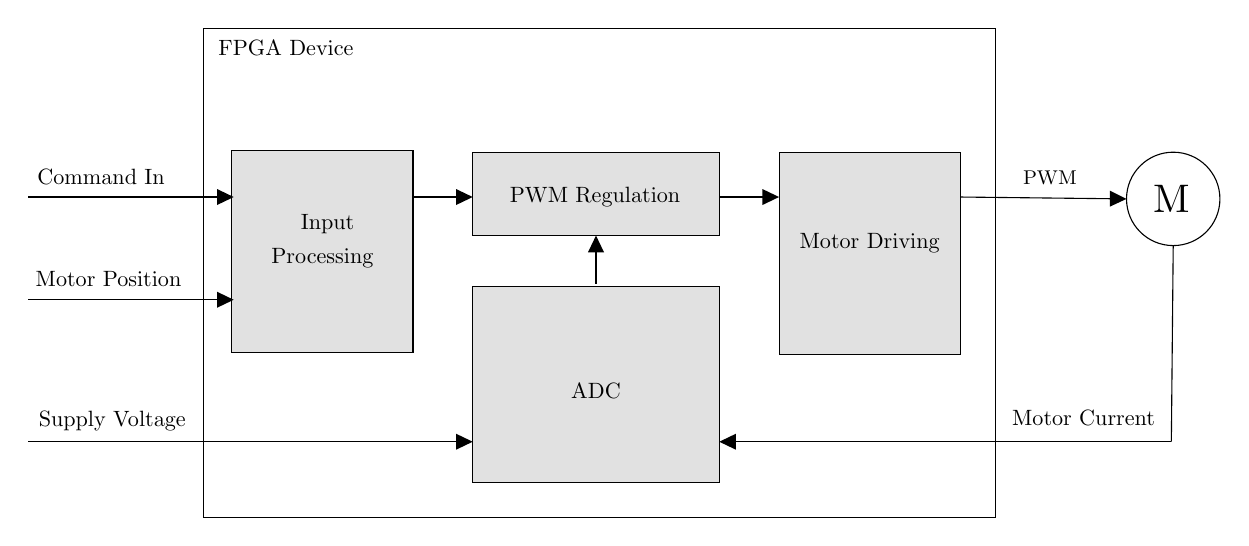
\begin{tikzpicture}[x=0.75pt,y=0.75pt,yscale=-0.9,xscale=0.9]
%uncomment if require: \path (0,290.6363525390625); %set diagram left start at 0, and has height of 290.6363525390625

%Shape: Circle [id:dp37060167234059627] 
\draw   (602,107) .. controls (602,93.19) and (613.19,82) .. (627,82) .. controls (640.81,82) and (652,93.19) .. (652,107) .. controls (652,120.81) and (640.81,132) .. (627,132) .. controls (613.19,132) and (602,120.81) .. (602,107) -- cycle ;

%Straight Lines [id:da8457845643324124] 
\draw    (513.05,106) -- (599,106.97) ;
\draw [shift={(602,107)}, rotate = 180.64] [fill={rgb, 255:red, 0; green, 0; blue, 0 }  ][line width=0.08]  [draw opacity=0] (8.93,-4.29) -- (0,0) -- (8.93,4.29) -- cycle    ;

%Shape: Rectangle [id:dp9895913562419061] 
\draw  [fill={rgb, 255:red, 225; green, 225; blue, 225 }  ,fill opacity=1 ] (416.05,82) -- (513.05,82) -- (513.05,190.36) -- (416.05,190.36) -- cycle ;
%Straight Lines [id:da89362591639862] 
\draw    (626,237) -- (387,237) ;
\draw [shift={(384,237)}, rotate = 360] [fill={rgb, 255:red, 0; green, 0; blue, 0 }  ][line width=0.08]  [draw opacity=0] (8.93,-4.29) -- (0,0) -- (8.93,4.29) -- cycle    ;

%Straight Lines [id:da3647004512136063] 
\draw    (626,237) -- (627,132) ;


%Shape: Rectangle [id:dp22253882061890917] 
\draw   (108.05,15.64) -- (532.05,15.64) -- (532.05,277.64) -- (108.05,277.64) -- cycle ;
%Straight Lines [id:da4479460701262754] 
\draw    (384.64,106) -- (413,106) ;
\draw [shift={(416,106)}, rotate = 180] [fill={rgb, 255:red, 0; green, 0; blue, 0 }  ][line width=0.08]  [draw opacity=0] (8.93,-4.29) -- (0,0) -- (8.93,4.29) -- cycle    ;

%Shape: Rectangle [id:dp7862653443183867] 
\draw  [fill={rgb, 255:red, 225; green, 225; blue, 225 }  ,fill opacity=1 ] (252,82) -- (384,82) -- (384,126.64) -- (252,126.64) -- cycle ;
%Shape: Rectangle [id:dp8459838496523577] 
\draw  [fill={rgb, 255:red, 225; green, 225; blue, 225 }  ,fill opacity=1 ] (123.05,81) -- (220.05,81) -- (220.05,189.36) -- (123.05,189.36) -- cycle ;
%Straight Lines [id:da5317523796080506] 
\draw    (318,129.64) -- (318,152.64) ;

\draw [shift={(318,126.64)}, rotate = 90] [fill={rgb, 255:red, 0; green, 0; blue, 0 }  ][line width=0.08]  [draw opacity=0] (8.93,-4.29) -- (0,0) -- (8.93,4.29) -- cycle    ;
%Straight Lines [id:da8756486664401073] 
\draw    (220.64,106) -- (249,106) ;
\draw [shift={(252,106)}, rotate = 180] [fill={rgb, 255:red, 0; green, 0; blue, 0 }  ][line width=0.08]  [draw opacity=0] (8.93,-4.29) -- (0,0) -- (8.93,4.29) -- cycle    ;

%Shape: Rectangle [id:dp2661938237798891] 
\draw  [fill={rgb, 255:red, 225; green, 225; blue, 225 }  ,fill opacity=1 ] (252,154) -- (384,154) -- (384,258.64) -- (252,258.64) -- cycle ;
%Straight Lines [id:da7659205141917105] 
\draw    (249,237) -- (14.05,237) ;

\draw [shift={(252,237)}, rotate = 180] [fill={rgb, 255:red, 0; green, 0; blue, 0 }  ][line width=0.08]  [draw opacity=0] (8.93,-4.29) -- (0,0) -- (8.93,4.29) -- cycle    ;
%Straight Lines [id:da5160015319494151] 
\draw    (121.05,161) -- (14.05,161) ;

\draw [shift={(124.05,161)}, rotate = 180] [fill={rgb, 255:red, 0; green, 0; blue, 0 }  ][line width=0.08]  [draw opacity=0] (8.93,-4.29) -- (0,0) -- (8.93,4.29) -- cycle    ;
%Straight Lines [id:da10479838194944624] 
\draw    (121.05,106) -- (14.05,106) ;

\draw [shift={(124.05,106)}, rotate = 180] [fill={rgb, 255:red, 0; green, 0; blue, 0 }  ][line width=0.08]  [draw opacity=0] (8.93,-4.29) -- (0,0) -- (8.93,4.29) -- cycle    ;

% Text Node
\draw (561,95.5) node  [scale=0.8] [align=left] {{\small PWM}};
% Text Node
\draw (626,107) node  [scale=1.44] [align=left] {M};
% Text Node
\draw (464.52,130.62) node  [scale=0.8] [align=left] {Motor Driving};
% Text Node
\draw (318,210) node  [scale=0.8] [align=left] {ADC};
% Text Node
\draw (579.02,224) node  [scale=0.8] [align=left] {Motor Current};
% Text Node
\draw (317.52,106) node  [scale=0.8] [align=left] {PWM Regulation};
% Text Node
\draw (171.52,129.62) node  [scale=0.8] [align=left] { \ \ \ \ Input \\Processing};
% Text Node
\draw (53.05,95) node  [scale=0.8] [align=left] {Command In};
% Text Node
\draw (57.05,150) node  [scale=0.8] [align=left] {Motor Position};
% Text Node
\draw (59.05,226) node  [scale=0.8] [align=left] {Supply Voltage};
% Text Node
\draw (152.05,26) node  [scale=0.8] [align=left] {FPGA Device};


\end{tikzpicture}

    \caption{High-level system architecture diagram showing system modules}
    \label{sys_architecture}
\end{figure}


%\subsection{Module Behaviours and Interactions}

The Input Processing module handles the command and position input. The module needs to analyse the values of each of the inputs and determine whether a movement is necessary. It should interpret the received commands and position to determine the direction of the movement if a movement is necessary. This module also controls the motor driving process which handles timings and stopping conditions.

The ADC module performs need to perform two measurements in order to provide voltage and current information to the PWM Regulation module. The supply voltage must be measured when the motor is not being driven. This allows the regulation process to limit the maximum PWM based on the supply voltage to prevent high currents. During motor control, the ADC must measure the motor current so that the PWM Regulation process can update the duty-cycle based on the response of the motor.

The PWM Regulation module calculates the required duty-cycle for motor driving. It does this by monitoring the motor current, calculated by the ADC, and adjusting the duty-cycle accordingly. The upper limit of the duty-cycles is determined by the supply voltage. This is to prevent higher voltages from over-accelerating the motor. The PWM module is also required for generating a PWM of the calculated duty-cycle value.

The motor driving module takes the PWM output by the regulation unit and supplies it to the correct motor driving transistors. The driving is performed by two IGBT / Thyristor pairs. This module needs to ensure the correct pair is driven based on the required direction of movement. It also performs the Thyristor and IGBT startup by driving them full for a given time specified in the requirements. The braking phase, also performed by the motor driving module, involves fully driving both IGBTs to stop the rotation of the motor. 





\section{Module Design and Implementation}

After the modules and the architecture have been defined, the V-model recommends performing module design. This process involves breaking down the module requirements into sub-modules which can then be designed in accordance to the V-model. For each of the four modules defined in the system architecture, the inputs, outputs and processing requirements are discussed. The implementation of the design is also presented for each module.

\subsection{Input Processing}

\begin{figure}[h]
\centering
\includegraphics[width=0.89\textwidth]{images/Positions.pdf}
\caption{Valid motor positions from original ATyS specification}
\label{motor_positions}
\end{figure}

% position design
The position of the motor has to be monitored continuously throughout the control process in order to determine whether the desired position has been reached. The position is read from a series of push-button switches. The valid motor positions can be seen in Figure \ref{motor_positions}. This diagram shows the three motor positions zero, one and two representing a connection between no sources, source one and source two respectively. The diagram also shows the readable intermediate positions. In total there are seven valid positions for the motor to be in. The position measurement needs to be filtered in order to debounce the signal, ensuring that only valid position changes are propagated through the system.

% position implementation
The existing acquisition method was used in this design to determine the position of the motor. There are four buttons read into the system, along with their inverse value to confirm the state of the button, in order to determine the position of the motor. The position acquisition process translates these into a commonly understood positional encoding. The code which performs this translation is shown in Appendix Item \ref{position-multiplexing-code}. This encoding scheme indicated the absolute and relative position (for example to the left of position zero). This allowed the required movement to be calculated more easily and requiring less logic. It also handles movement from intermediate positions. 

% command design
For this prototype, only the customer command interface is being considered. This means that commands are supplied by stimulating a voltage input. There are three possible commands: go to position zero, go to position one and go to position two. Each of these should be processed and the motor should move to the position indicated by the command input.
% command implementation
The command is encoded in a similar way to the position. The required movement is encoded as a position in order to perform a comparison and calculate the required movement. This also allows the desired position to be determined so that the system can stop the motor when the position is reached. 

% debounce implementation
A shared debouncing process was used for both the position acquisition and the command interpreting in order to prevent glitches in the reading of inputs. It uses a shift register and comparison in order to ensure the input value is consistent. This shift register is currently only three bits; however, this value can be expanded to allow for more sophisticated debouncing. In this application, it was found that three bits was sufficient to avoid misreadings.

% launch system / move design and implementation
The device must interpret from the current position and the command which has been supplied whether a movement is necessary. It uses the shared position encoding scheme of the command and the position reading to compare the value and determine a direction of movement unless they are the same then no movement is required. After determining the required position, it provides directional information to the modules which perform the movement. The code which performs this decision-making logic is shown in Appendix Item \ref{input-processing-code}. The position must then be continually monitored to detect when the motor movement has been reached. Once this module detects the position has been reached, it must signal this to the movement modules to halt the motion. Taken from the specification, this module will signal the motor to stop if the position has not been reached after five seconds. 

\subsection{ADC}

There are two values which have to be measured by the processor: the supply voltage and the motor current. These allow for the accurate control of the motor. The value of the supply voltage determines the maximum duty-cycle of the PWM which drives the motor. This is to prevent over-driving which could cause current spikes. This value does not need to be updated during the motor driving phase. The motor current is used to regulate the PWM value to allow for optimal control of the motor during the motor driving phase. 

The ADC which has been adopted in this FPGA is a sigma-delta ADC implemented in VHDL. This ADC has been implemented by Lattice Semiconductor and the structure of it is shown in Figure \ref{adc_schematic}. Each of the modules is implemented internally to the FPGA with the exception of the RC Network and the Comparator which are implemented on the peripheral of the FPGA. Since these measurements are never taken at the same time and in the interest of saving space on the FPGA, these two values are measured using the same ADC. The value measurement of the Lattice ADC is multiplexed to allow each of the values to be measured. The implementation code which performs this input multiplexing is shown in Appendix Item \ref{adc-multiplexing-code}.

\begin{figure}[h]
\centering


\tikzset{every picture/.style={line width=0.75pt}} %set default line width to 0.75pt        

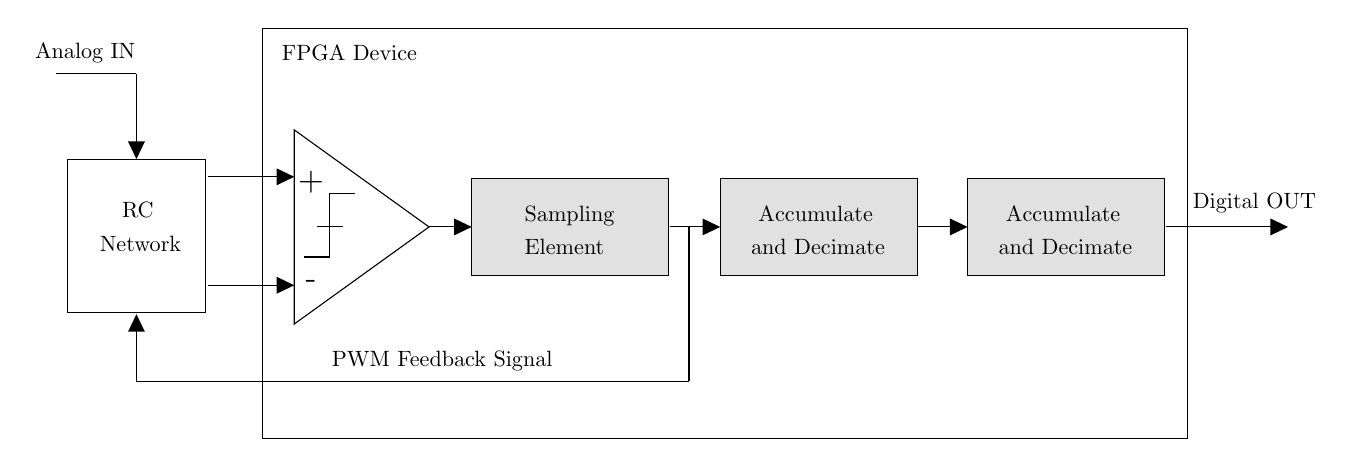
\begin{tikzpicture}[x=0.75pt,y=0.75pt,yscale=-0.95,xscale=0.95]
%uncomment if require: \path (0,300); %set diagram left start at 0, and has height of 300

%Shape: Rectangle [id:dp9604023161903008] 
\draw   (124.05,6.64) -- (593.05,6.64) -- (593.05,214.64) -- (124.05,214.64) -- cycle ;
%Straight Lines [id:da9484599770004658] 
\draw    (330.44,107.42) -- (353.05,107.42) ;
\draw [shift={(356.05,107.42)}, rotate = 180] [fill={rgb, 255:red, 0; green, 0; blue, 0 }  ][line width=0.08]  [draw opacity=0] (8.93,-4.29) -- (0,0) -- (8.93,4.29) -- cycle    ;

%Shape: Rectangle [id:dp7904328314933544] 
\draw  [fill={rgb, 255:red, 225; green, 225; blue, 225 }  ,fill opacity=1 ] (230,82.9) -- (330.05,82.9) -- (330.05,131.94) -- (230,131.94) -- cycle ;

%Straight Lines [id:da4819176246297532] 
\draw    (208.39,107.42) -- (227.05,107.42) ;
\draw [shift={(230.05,107.42)}, rotate = 180] [fill={rgb, 255:red, 0; green, 0; blue, 0 }  ][line width=0.08]  [draw opacity=0] (8.93,-4.29) -- (0,0) -- (8.93,4.29) -- cycle    ;

%Straight Lines [id:da24497687439569482] 
\draw    (60,70) -- (60,29.64) ;

\draw [shift={(60,73)}, rotate = 270] [fill={rgb, 255:red, 0; green, 0; blue, 0 }  ][line width=0.08]  [draw opacity=0] (8.93,-4.29) -- (0,0) -- (8.93,4.29) -- cycle    ;
%Straight Lines [id:da9302636844153138] 
\draw    (137.05,137) -- (96.05,137) ;

\draw [shift={(140.05,137)}, rotate = 180] [fill={rgb, 255:red, 0; green, 0; blue, 0 }  ][line width=0.08]  [draw opacity=0] (8.93,-4.29) -- (0,0) -- (8.93,4.29) -- cycle    ;
%Straight Lines [id:da2916048291189839] 
\draw    (137.05,82) -- (96.05,82) ;

\draw [shift={(140.05,82)}, rotate = 180] [fill={rgb, 255:red, 0; green, 0; blue, 0 }  ][line width=0.08]  [draw opacity=0] (8.93,-4.29) -- (0,0) -- (8.93,4.29) -- cycle    ;
%Shape: Triangle [id:dp8965603701252123] 
\draw   (208.39,107.42) -- (140.05,156.64) -- (140.05,58.2) -- cycle ;
%Shape: Rectangle [id:dp2519733387539336] 
\draw  [fill={rgb, 255:red, 225; green, 225; blue, 225 }  ,fill opacity=1 ] (356,82.9) -- (456.05,82.9) -- (456.05,131.94) -- (356,131.94) -- cycle ;

%Straight Lines [id:da7883255728251393] 
\draw    (456.44,107.42) -- (478.52,107.42) ;
\draw [shift={(481.52,107.42)}, rotate = 180] [fill={rgb, 255:red, 0; green, 0; blue, 0 }  ][line width=0.08]  [draw opacity=0] (8.93,-4.29) -- (0,0) -- (8.93,4.29) -- cycle    ;

%Shape: Rectangle [id:dp34966320633084025] 
\draw  [fill={rgb, 255:red, 225; green, 225; blue, 225 }  ,fill opacity=1 ] (481.5,82.9) -- (581.55,82.9) -- (581.55,131.94) -- (481.5,131.94) -- cycle ;

%Shape: Rectangle [id:dp20202629131702943] 
\draw   (25,73) -- (95,73) -- (95,150.64) -- (25,150.64) -- cycle ;
%Straight Lines [id:da3350824826473666] 
\draw    (19.05,29.64) -- (60,29.64) ;


%Straight Lines [id:da8160728779847974] 
\draw    (582.05,107.42) -- (641.05,107.42) ;
\draw [shift={(644.05,107.42)}, rotate = 180] [fill={rgb, 255:red, 0; green, 0; blue, 0 }  ][line width=0.08]  [draw opacity=0] (8.93,-4.29) -- (0,0) -- (8.93,4.29) -- cycle    ;

%Straight Lines [id:da4116203957240303] 
\draw    (158.05,90.27) -- (158.05,122.64) ;


%Straight Lines [id:da2244964116397019] 
\draw    (145.05,122.64) -- (158.05,122.64) ;


%Straight Lines [id:da41850801552553585] 
\draw    (158.05,90.27) -- (171.05,90.27) ;


%Straight Lines [id:da28517286500051164] 
\draw    (151.71,107.42) -- (164.71,107.42) ;


%Straight Lines [id:da7677560417405613] 
\draw    (60,154.64) -- (60,185.64) ;

\draw [shift={(60,151.64)}, rotate = 90] [fill={rgb, 255:red, 0; green, 0; blue, 0 }  ][line width=0.08]  [draw opacity=0] (8.93,-4.29) -- (0,0) -- (8.93,4.29) -- cycle    ;
%Straight Lines [id:da2763081409638619] 
\draw    (340.24,107.42) -- (340.24,185.64) ;


%Straight Lines [id:da4366815569167197] 
\draw    (340.24,185.64) -- (60,185.64) ;



% Text Node
\draw (62.05,107.42) node  [scale=0.8] [align=left] { \ \ \ RC \\Network};
% Text Node
\draw (215.05,175.14) node  [scale=0.8] [align=left] {PWM Feedback Signal};
% Text Node
\draw (168.05,19) node  [scale=0.8] [align=left] {FPGA Device};
% Text Node
\draw (279.66,109.27) node  [scale=0.8] [align=left] {Sampling\\ Element};
% Text Node
\draw (405.66,109.27) node  [scale=0.8] [align=left] { \ Accumulate\\and Decimate};
% Text Node
\draw (531.16,109.27) node  [scale=0.8] [align=left] { \ Accumulate\\and Decimate};
% Text Node
\draw (34,19.42) node  [scale=0.8] [align=left] {Analog IN};
% Text Node
\draw (627,95.05) node  [scale=0.8] [align=left] {Digital OUT};
% Text Node
\draw (148.55,84.55) node  [scale=1.2] [align=left] {+};
% Text Node
\draw (148.55,135.14) node   [align=left] {{\large -}};


\end{tikzpicture}

\caption{Schematic of the ADC obtained from Lattice\cite{LatticeADC}}
\label{adc_schematic}
\end{figure}



\subsection{PWM Regulation}
% combine with motor drive?

%\subsection{Motor Current Regulation}
The regulation of PWM limits the motor current which prevents dangerous current spikes. The measured motor current should be controlled against a predefined reference\cite{Aime}. The duty-cycle of the applied PWM can be regulated in order to control the speed of the motor\cite{Sathyan}. Duty-cycle controlled motor drive simplifies the regulation of motor speed\cite{Sathyan}.
From the specification, the PWM needs to be regulated using a simple proportional control based on the motor current. Linear regulation of PWM is a simple and efficient control system\cite{Sathyan}. 

Since the motor is being driven by a PWM signal, the current spikes up when the PWM is high and it drops when the PWM is low. In order to filter out the effect of this and get an average reading, the current should be measured in the middle of the PWM on-time. This allows the value to be averaged and provides a consistent reading.
FPGAs are able to synchronise the measurement of the current and the PWM duty-cycle in order to obtain a more accurate measurement\cite{MonmassonDesign, Gomes}. This current value is used to update the PWM value to allow for optimal control.


The PWM regulation scheme was implemented using a first-order proportional control scheme shown in Figure \ref{motor_control_loop}. 
This control scheme was chosen because it can easily be implemented in a VHDL design using a series of basic calculations and shifts. Techniques such as fixed point arithmetic can be used to implement more complex control systems. However, a first-order scheme was found to be efficient and sufficient for this application.
In this control scheme, the current value measured by the ADC is compared against the nominal value of 1A. This error is then translated into an error in PWM duty-cycle by applying a gain. Then, if the regulation is enabled in the control phase, the PWM duty-cycle value is updated. The value is truncated to ensure that it stays between the valid boundary set by the minimum and maximum values. The code which implements this PWM regulation process is shown in Appendix Item \ref{pwm-regulation-code}. The calculated value is provided to the PWM generator which translates this value into a PWM signal with a duty-cycle specified by the regulation scheme. The PWM Generator module triggers the current measurement at the midpoint of the duty-cycle in order to smooth the current measurement, as mentioned above. When triggered, the ADC value is taken in and used in the comparison. The value updates at 1kHz, once for every PWM cycle.


\begin{figure}
    \centering
    

\tikzset{every picture/.style={line width=0.75pt}} %set default line width to 0.75pt        

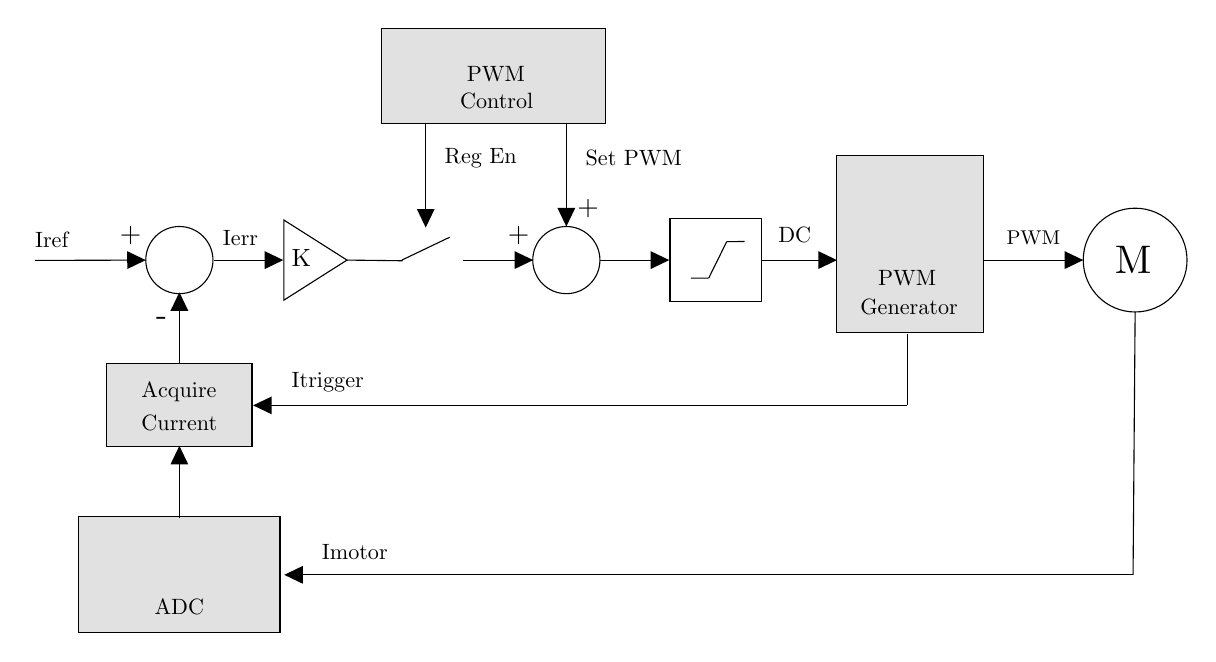
\begin{tikzpicture}[x=0.75pt,y=0.75pt,yscale=-1,xscale=1]
%uncomment if require: \path (0,300); %set diagram left start at 0, and has height of 300

%Shape: Circle [id:dp75942846606901] 
\draw   (130.33,112) .. controls (130.33,103.06) and (137.58,95.82) .. (146.52,95.82) .. controls (155.45,95.82) and (162.7,103.06) .. (162.7,112) .. controls (162.7,120.94) and (155.45,128.18) .. (146.52,128.18) .. controls (137.58,128.18) and (130.33,120.94) .. (130.33,112) -- cycle ;
%Straight Lines [id:da27986909082362965] 
\draw    (146.52,162.21) -- (146.52,130.5) ;
\draw [shift={(146.52,127.5)}, rotate = 450] [fill={rgb, 255:red, 0; green, 0; blue, 0 }  ][line width=0.08]  [draw opacity=0] (8.93,-4.29) -- (0,0) -- (8.93,4.29) -- cycle    ;

%Straight Lines [id:da6600230288463764] 
\draw    (77.05,112.16) -- (127.33,112.01) ;
\draw [shift={(130.33,112)}, rotate = 539.8299999999999] [fill={rgb, 255:red, 0; green, 0; blue, 0 }  ][line width=0.08]  [draw opacity=0] (8.93,-4.29) -- (0,0) -- (8.93,4.29) -- cycle    ;

%Shape: Rectangle [id:dp714942454713728] 
\draw  [fill={rgb, 255:red, 225; green, 225; blue, 225 }  ,fill opacity=1 ] (463,61.52) -- (534.05,61.52) -- (534.05,147) -- (463,147) -- cycle ;
%Shape: Triangle [id:dp4366865800134343] 
\draw   (227.28,112) -- (196.84,131.32) -- (196.84,92.68) -- cycle ;
%Straight Lines [id:da3696616039173719] 
\draw    (227.28,112) -- (254.05,112.32) ;


%Straight Lines [id:da9691180490319533] 
\draw    (253.71,112) -- (276.71,101) ;


%Straight Lines [id:da2520686052851293] 
\draw    (283.36,112) -- (313.98,112) ;
\draw [shift={(316.98,112)}, rotate = 180] [fill={rgb, 255:red, 0; green, 0; blue, 0 }  ][line width=0.08]  [draw opacity=0] (8.93,-4.29) -- (0,0) -- (8.93,4.29) -- cycle    ;

%Shape: Rectangle [id:dp24319017769923046] 
\draw   (382.9,92) -- (427,92) -- (427,132) -- (382.9,132) -- cycle ;
%Straight Lines [id:da7467210515424787] 
\draw    (401.56,120.66) -- (410.24,103.1) ;


%Straight Lines [id:da9410268597126219] 
\draw    (410.24,103.1) -- (418.83,103.05) ;


%Straight Lines [id:da8375418901691511] 
\draw    (392.96,120.71) -- (401.56,120.66) ;



%Straight Lines [id:da7342599903712179] 
\draw    (427.34,112) -- (460.34,112) ;
\draw [shift={(463.34,112)}, rotate = 180] [fill={rgb, 255:red, 0; green, 0; blue, 0 }  ][line width=0.08]  [draw opacity=0] (8.93,-4.29) -- (0,0) -- (8.93,4.29) -- cycle    ;

%Straight Lines [id:da296371673100567] 
\draw    (265.21,46.09) -- (265.21,93.32) ;
\draw [shift={(265.21,96.32)}, rotate = 270] [fill={rgb, 255:red, 0; green, 0; blue, 0 }  ][line width=0.08]  [draw opacity=0] (8.93,-4.29) -- (0,0) -- (8.93,4.29) -- cycle    ;

%Shape: Rectangle [id:dp9289257972427081] 
\draw  [fill={rgb, 255:red, 225; green, 225; blue, 225 }  ,fill opacity=1 ] (244.05,0.29) -- (351.94,0.29) -- (351.94,46) -- (244.05,46) -- cycle ;
%Shape: Circle [id:dp49019498566872044] 
\draw   (316.78,112) .. controls (316.78,103.06) and (324.02,95.82) .. (332.96,95.82) .. controls (341.9,95.82) and (349.14,103.06) .. (349.14,112) .. controls (349.14,120.94) and (341.9,128.18) .. (332.96,128.18) .. controls (324.02,128.18) and (316.78,120.94) .. (316.78,112) -- cycle ;
%Straight Lines [id:da140038158148579] 
\draw    (332.96,46.09) -- (332.96,92.82) ;
\draw [shift={(332.96,95.82)}, rotate = 270] [fill={rgb, 255:red, 0; green, 0; blue, 0 }  ][line width=0.08]  [draw opacity=0] (8.93,-4.29) -- (0,0) -- (8.93,4.29) -- cycle    ;

%Straight Lines [id:da6535254105925976] 
\draw    (162.96,112) -- (193.58,112) ;
\draw [shift={(196.58,112)}, rotate = 180] [fill={rgb, 255:red, 0; green, 0; blue, 0 }  ][line width=0.08]  [draw opacity=0] (8.93,-4.29) -- (0,0) -- (8.93,4.29) -- cycle    ;

%Straight Lines [id:da8262984100189177] 
\draw    (348.94,112) -- (379.55,112) ;
\draw [shift={(382.55,112)}, rotate = 180] [fill={rgb, 255:red, 0; green, 0; blue, 0 }  ][line width=0.08]  [draw opacity=0] (8.93,-4.29) -- (0,0) -- (8.93,4.29) -- cycle    ;

%Shape: Circle [id:dp25249517388379217] 
\draw   (582,112) .. controls (582,98.19) and (593.19,87) .. (607,87) .. controls (620.81,87) and (632,98.19) .. (632,112) .. controls (632,125.81) and (620.81,137) .. (607,137) .. controls (593.19,137) and (582,125.81) .. (582,112) -- cycle ;

%Straight Lines [id:da6638712668031186] 
\draw    (534.34,112) -- (579,112) ;
\draw [shift={(582,112)}, rotate = 180] [fill={rgb, 255:red, 0; green, 0; blue, 0 }  ][line width=0.08]  [draw opacity=0] (8.93,-4.29) -- (0,0) -- (8.93,4.29) -- cycle    ;

%Shape: Rectangle [id:dp6025687451357558] 
\draw  [fill={rgb, 255:red, 225; green, 225; blue, 225 }  ,fill opacity=1 ] (111.52,162) -- (181.52,162) -- (181.52,202) -- (111.52,202) -- cycle ;
%Shape: Rectangle [id:dp6368460798569435] 
\draw  [fill={rgb, 255:red, 225; green, 225; blue, 225 }  ,fill opacity=1 ] (98.03,235.64) -- (195,235.64) -- (195,291.64) -- (98.03,291.64) -- cycle ;
%Straight Lines [id:da3095935870834763] 
\draw    (146.52,236.21) -- (146.52,204.5) ;
\draw [shift={(146.52,201.5)}, rotate = 450] [fill={rgb, 255:red, 0; green, 0; blue, 0 }  ][line width=0.08]  [draw opacity=0] (8.93,-4.29) -- (0,0) -- (8.93,4.29) -- cycle    ;

%Straight Lines [id:da7119757417617545] 
\draw    (497.15,182) -- (185.05,182) ;
\draw [shift={(182.05,182)}, rotate = 360] [fill={rgb, 255:red, 0; green, 0; blue, 0 }  ][line width=0.08]  [draw opacity=0] (8.93,-4.29) -- (0,0) -- (8.93,4.29) -- cycle    ;

%Straight Lines [id:da555961758391875] 
\draw    (606,263.64) -- (200.05,263.64) ;
\draw [shift={(197.05,263.64)}, rotate = 360] [fill={rgb, 255:red, 0; green, 0; blue, 0 }  ][line width=0.08]  [draw opacity=0] (8.93,-4.29) -- (0,0) -- (8.93,4.29) -- cycle    ;

%Straight Lines [id:da5618757081316239] 
\draw    (606,263.64) -- (607,137) ;


%Straight Lines [id:da9238020071399877] 
\draw    (497.15,182) -- (497.15,147.64) ;



% Text Node
\draw (123,100.16) node  [scale=1] [align=left] {+};
% Text Node
\draw (138.02,140) node  [scale=1.2] [align=left] {\mbox{-}};
% Text Node
\draw (85,102) node  [scale=0.8] [align=left] {Iref};
% Text Node
\draw (205.21,111) node  [scale=0.9] [align=left] {K};
% Text Node
\draw (497.15,120.52) node  [scale=0.8] [align=left] {PWM};
% Text Node
\draw (498.1,134.52) node  [scale=0.8] [align=left] {Generator};
% Text Node
\draw (299.42,35.09) node  [scale=0.8] [align=left] {Control};
% Text Node
\draw (298.99,22.49) node  [scale=0.8] [align=left] {PWM};
% Text Node
\draw (558,101.16) node  [scale=0.8] [align=left] {{\small PWM}};
% Text Node
\draw (606,112) node  [scale=1.44] [align=left] {M};
% Text Node
\draw (443,100) node  [scale=0.8] [align=left] {DC};
% Text Node
\draw (146.52,182.33) node  [scale=0.8] [align=left] {Acquire\\Current};
% Text Node
\draw (146.52,279) node  [scale=0.8] [align=left] {ADC};
% Text Node
\draw (310,100.16) node  [scale=1] [align=left] {+};
% Text Node
\draw (343.46,87.16) node  [scale=1] [align=left] {+};
% Text Node
\draw (365.46,63) node  [scale=0.8] [align=left] {Set PWM};
% Text Node
\draw (291.71,63) node  [scale=0.8] [align=left] {Reg En};
% Text Node
\draw (176,101.16) node  [scale=0.8] [align=left] {Ierr};
% Text Node
\draw (218,171) node  [scale=0.8] [align=left] {Itrigger};
% Text Node
\draw (231.02,252.64) node  [scale=0.8] [align=left] {Imotor};


\end{tikzpicture}

    \caption{PWM regulation process control loop}
    \label{motor_control_loop}
\end{figure}

This control scheme was used to map to the response from the microcontroller-based regulation scheme. The output of the regulation scheme was analysed and modelled. The microcontroller output that was analysed and modelled is shown in Section \ref{regulation-results}. It was found to be a simple proportional controller. The simple control response was modified to include processes outlined in the requirements. For example, the current is acquired half-way through the on-time using a trigger from the PWM duty-cycle. Truncation was performed on the calculated value to ensure that it stayed between the defined minimum and the calculated maximum.

\subsection{Motor Driving}

The motor is driven using an H-bridge scheme consisting of two IGBT and Thyristor pairs. This circuit can be seen in Figure \ref{motor_control_circuit}. The motor drive module has to multiplex the PWM and control signals generated by the regulation phase to drive the correct IGBTs and Thyristors. The driving sequence is being modelled on the current set of requirements. It contains several discrete stages in order to drive the Thyristors and IGBTs to move the motor to the required position.

\begin{figure}
\centering


\tikzset{every picture/.style={line width=0.75pt}} %set default line width to 0.75pt        

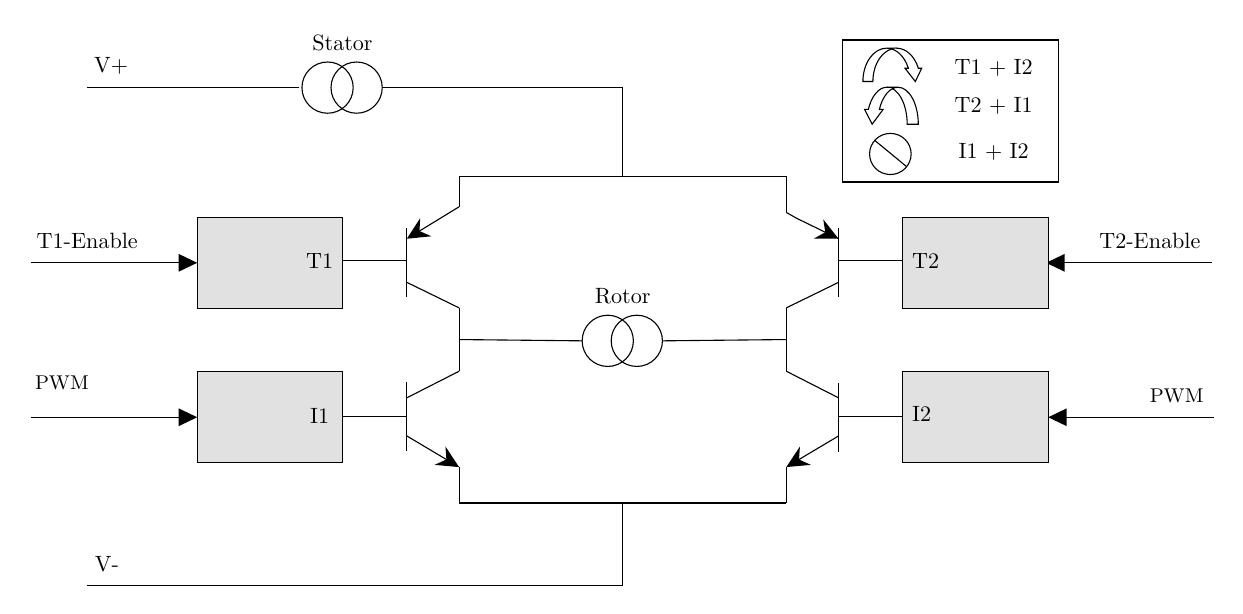
\begin{tikzpicture}[x=0.75pt,y=0.75pt,yscale=-1,xscale=1]
%uncomment if require: \path (0,300); %set diagram left start at 0, and has height of 300

%Straight Lines [id:da9221466297195395] 
\draw    (189.05,188.5) -- (158.05,188.5) ;


%Straight Lines [id:da5673743870695822] 
\draw    (8.05,114.59) -- (85.05,114.59) ;
\draw [shift={(88.05,114.59)}, rotate = 180] [fill={rgb, 255:red, 0; green, 0; blue, 0 }  ][line width=0.08]  [draw opacity=0] (8.93,-4.29) -- (0,0) -- (8.93,4.29) -- cycle    ;

%Straight Lines [id:da5344017083576562] 
\draw    (8.05,189) -- (85.05,189) ;
\draw [shift={(88.05,189)}, rotate = 180] [fill={rgb, 255:red, 0; green, 0; blue, 0 }  ][line width=0.08]  [draw opacity=0] (8.93,-4.29) -- (0,0) -- (8.93,4.29) -- cycle    ;

%Straight Lines [id:da4468699428839338] 
\draw    (214.22,73) -- (214.22,87.6) ;


%Straight Lines [id:da26254747962825764] 
\draw    (214.22,87.6) -- (191.6,101.43) ;
\draw [shift={(189.05,103)}, rotate = 328.53999999999996] [fill={rgb, 255:red, 0; green, 0; blue, 0 }  ][line width=0.08]  [draw opacity=0] (10.72,-5.15) -- (0,0) -- (10.72,5.15) -- (7.12,0) -- cycle    ;

%Straight Lines [id:da5823961798906938] 
\draw    (428.05,188.5) -- (397.05,188.5) ;


%Straight Lines [id:da29909831649241614] 
\draw    (428.05,113.5) -- (397.05,113.5) ;


%Straight Lines [id:da2356065415871993] 
\draw    (189.05,113.5) -- (158.05,113.5) ;


%Straight Lines [id:da30663699958544943] 
\draw    (189.05,98) -- (189.05,131.18) ;


%Straight Lines [id:da31696707767211185] 
\draw    (397.05,98) -- (397.05,131.18) ;


%Straight Lines [id:da673348118293702] 
\draw    (500.05,114.59) -- (577.05,114.59) ;

\draw [shift={(497.05,114.59)}, rotate = 0] [fill={rgb, 255:red, 0; green, 0; blue, 0 }  ][line width=0.08]  [draw opacity=0] (8.93,-4.29) -- (0,0) -- (8.93,4.29) -- cycle    ;
%Straight Lines [id:da3029592242109622] 
\draw    (501.05,189) -- (578.05,189) ;

\draw [shift={(498.05,189)}, rotate = 0] [fill={rgb, 255:red, 0; green, 0; blue, 0 }  ][line width=0.08]  [draw opacity=0] (8.93,-4.29) -- (0,0) -- (8.93,4.29) -- cycle    ;
%Straight Lines [id:da8114410961824066] 
\draw    (371.87,90.3) -- (376.68,93.04) -- (394.35,101.68) ;
\draw [shift={(397.05,103)}, rotate = 206.07] [fill={rgb, 255:red, 0; green, 0; blue, 0 }  ][line width=0.08]  [draw opacity=0] (10.72,-5.15) -- (0,0) -- (10.72,5.15) -- (7.12,0) -- cycle    ;

%Straight Lines [id:da20108401284003996] 
\draw    (371.87,73) -- (371.87,90.3) ;


%Straight Lines [id:da8481295471076566] 
\draw    (371.87,73) -- (214.22,73) ;


%Shape: Circle [id:dp10268436833983152] 
\draw   (273.51,152.18) .. controls (273.51,145.37) and (279.03,139.84) .. (285.85,139.84) .. controls (292.66,139.84) and (298.19,145.37) .. (298.19,152.18) .. controls (298.19,159) and (292.66,164.52) .. (285.85,164.52) .. controls (279.03,164.52) and (273.51,159) .. (273.51,152.18) -- cycle ;
%Shape: Circle [id:dp39801516955430727] 
\draw   (287.51,152.18) .. controls (287.51,145.37) and (293.03,139.84) .. (299.85,139.84) .. controls (306.66,139.84) and (312.19,145.37) .. (312.19,152.18) .. controls (312.19,159) and (306.66,164.52) .. (299.85,164.52) .. controls (293.03,164.52) and (287.51,159) .. (287.51,152.18) -- cycle ;

%Straight Lines [id:da726831823671015] 
\draw    (189.05,124) -- (214.22,136.3) ;


%Straight Lines [id:da778435519184604] 
\draw    (371.87,136.3) -- (397.05,124) ;


%Straight Lines [id:da4015757785120837] 
\draw    (189.05,171.91) -- (189.05,205.09) ;


%Straight Lines [id:da23166080135755474] 
\draw    (397.05,172.41) -- (397.05,205.59) ;


%Straight Lines [id:da7946452898081748] 
\draw    (189.05,179.64) -- (214.22,166.82) ;


%Straight Lines [id:da2217710859730495] 
\draw    (371.87,166.82) -- (397.05,179.64) ;


%Straight Lines [id:da5050058101228307] 
\draw    (214.22,136.3) -- (214.22,166.82) ;


%Straight Lines [id:da07368058014858048] 
\draw    (371.87,136.3) -- (371.87,166.82) ;


%Straight Lines [id:da4463883229770369] 
\draw    (214.22,151.56) -- (273.51,152.18) ;


%Straight Lines [id:da606524752619622] 
\draw    (312.19,152.18) -- (371.87,151.56) ;


%Straight Lines [id:da43391584718083376] 
\draw    (189.05,198) -- (211.64,211.46) ;
\draw [shift={(214.22,213)}, rotate = 210.79] [fill={rgb, 255:red, 0; green, 0; blue, 0 }  ][line width=0.08]  [draw opacity=0] (10.72,-5.15) -- (0,0) -- (10.72,5.15) -- (7.12,0) -- cycle    ;

%Straight Lines [id:da6840402308453948] 
\draw    (397.05,198) -- (374.45,211.46) ;
\draw [shift={(371.87,213)}, rotate = 329.21000000000004] [fill={rgb, 255:red, 0; green, 0; blue, 0 }  ][line width=0.08]  [draw opacity=0] (10.72,-5.15) -- (0,0) -- (10.72,5.15) -- (7.12,0) -- cycle    ;

%Straight Lines [id:da14157911992399308] 
\draw    (371.87,230.3) -- (214.22,230.3) ;


%Straight Lines [id:da9684058826846] 
\draw    (371.87,213) -- (371.87,230.3) ;


%Straight Lines [id:da027240572979521538] 
\draw    (214.22,213) -- (214.22,230.3) ;


%Shape: Circle [id:dp751541628776144] 
\draw   (138.51,30.18) .. controls (138.51,23.37) and (144.03,17.84) .. (150.85,17.84) .. controls (157.66,17.84) and (163.19,23.37) .. (163.19,30.18) .. controls (163.19,37) and (157.66,42.52) .. (150.85,42.52) .. controls (144.03,42.52) and (138.51,37) .. (138.51,30.18) -- cycle ;
%Shape: Circle [id:dp12782068359122056] 
\draw   (152.51,30.18) .. controls (152.51,23.37) and (158.03,17.84) .. (164.85,17.84) .. controls (171.66,17.84) and (177.19,23.37) .. (177.19,30.18) .. controls (177.19,37) and (171.66,42.52) .. (164.85,42.52) .. controls (158.03,42.52) and (152.51,37) .. (152.51,30.18) -- cycle ;

%Straight Lines [id:da9745722307494478] 
\draw    (293.05,30.18) -- (177.19,30.18) ;


%Straight Lines [id:da9525535594657324] 
\draw    (293.05,30.18) -- (293.05,73) ;


%Straight Lines [id:da7344305010710814] 
\draw    (137.05,30.18) -- (35.05,30.18) ;


%Straight Lines [id:da5373673836671371] 
\draw    (293.05,270.18) -- (35.05,270.18) ;


%Straight Lines [id:da8535356105812089] 
\draw    (293.05,230.3) -- (293.05,270.18) ;


%Curve Right Arrow [id:dp07248280783179872] 
\draw  [fill={rgb, 255:red, 255; green, 255; blue, 255 }  ,fill opacity=1 ] (425.02,11.18) .. controls (418.72,11.18) and (413.6,18.38) .. (413.6,27.25) -- (408.78,27.25) .. controls (408.78,18.38) and (413.89,11.18) .. (420.2,11.18) ;\draw  [fill={rgb, 255:red, 255; green, 255; blue, 255 }  ,fill opacity=1 ] (420.2,11.18) .. controls (424.88,11.18) and (428.9,15.15) .. (430.67,20.83) -- (429.06,20.83) -- (434.03,27.25) -- (437.1,20.83) -- (435.49,20.83) .. controls (433.73,15.15) and (429.7,11.18) .. (425.02,11.18)(420.2,11.18) -- (425.02,11.18) ;
%Curve Left Arrow [id:dp35549290685095736] 
\draw  [fill={rgb, 255:red, 255; green, 255; blue, 255 }  ,fill opacity=1 ] (425.68,30) .. controls (431.08,30) and (435.46,37.98) .. (435.46,47.82) -- (430.11,47.82) .. controls (430.11,37.98) and (425.74,30) .. (420.34,30) ;\draw  [fill={rgb, 255:red, 255; green, 255; blue, 255 }  ,fill opacity=1 ] (420.34,30) .. controls (416.33,30) and (412.89,34.4) .. (411.38,40.69) -- (409.6,40.69) -- (413.24,47.82) -- (418.51,40.69) -- (416.72,40.69) .. controls (418.23,34.4) and (421.68,30) .. (425.68,30)(420.34,30) -- (425.68,30) ;
%Shape: Ellipse [id:dp4400378009685477] 
\draw   (411.99,62.15) .. controls (411.99,56.67) and (416.47,52.24) .. (422,52.24) .. controls (427.53,52.24) and (432.02,56.67) .. (432.02,62.15) .. controls (432.02,67.62) and (427.53,72.06) .. (422,72.06) .. controls (416.47,72.06) and (411.99,67.62) .. (411.99,62.15) -- cycle ;
%Straight Lines [id:da593928177084287] 
\draw    (414.32,55.48) -- (429.89,68.29) ;


%Shape: Rectangle [id:dp9415861976749436] 
\draw   (399.03,7.25) -- (503.05,7.25) -- (503.05,75.64) -- (399.03,75.64) -- cycle ;
%Shape: Rectangle [id:dp9348588765520855] 
\draw  [fill={rgb, 255:red, 225; green, 225; blue, 225 }  ,fill opacity=1 ] (88.05,92.73) -- (158.05,92.73) -- (158.05,136.45) -- (88.05,136.45) -- cycle ;
%Shape: Rectangle [id:dp09631198686380071] 
\draw  [fill={rgb, 255:red, 225; green, 225; blue, 225 }  ,fill opacity=1 ] (428.05,167.14) -- (498.05,167.14) -- (498.05,210.86) -- (428.05,210.86) -- cycle ;
%Shape: Rectangle [id:dp45121828009239695] 
\draw  [fill={rgb, 255:red, 225; green, 225; blue, 225 }  ,fill opacity=1 ] (428.05,92.73) -- (498.05,92.73) -- (498.05,136.45) -- (428.05,136.45) -- cycle ;
%Shape: Rectangle [id:dp41843258071231526] 
\draw  [fill={rgb, 255:red, 225; green, 225; blue, 225 }  ,fill opacity=1 ] (88.05,167.14) -- (158.05,167.14) -- (158.05,210.86) -- (88.05,210.86) -- cycle ;

% Text Node
\draw (559.94,178.5) node  [scale=0.8] [align=left] {{\small PWM}};
% Text Node
\draw (547.05,104.09) node  [scale=0.8] [align=left] {T2-Enable};
% Text Node
\draw (22.87,172.5) node  [scale=0.8] [align=left] {{\small PWM}};
% Text Node
\draw (35.05,104.09) node  [scale=0.8] [align=left] {T1-Enable};
% Text Node
\draw (147.05,113.5) node  [scale=0.8] [align=left] {T1};
% Text Node
\draw (439.05,113.5) node  [scale=0.8] [align=left] {T2};
% Text Node
\draw (147.05,188.5) node  [scale=0.8] [align=left] {I1};
% Text Node
\draw (437.05,187.5) node  [scale=0.8] [align=left] {I2};
% Text Node
\draw (46.55,19.68) node  [scale=0.8] [align=left] {V+};
% Text Node
\draw (44.55,259.68) node  [scale=0.8] [align=left] {V-};
% Text Node
\draw (293.05,130.5) node  [scale=0.8] [align=left] {Rotor};
% Text Node
\draw (158.05,8.5) node  [scale=0.8] [align=left] {Stator};
% Text Node
\draw (471.78,20.52) node  [scale=0.8] [align=left] {T1 + I2};
% Text Node
\draw (471.78,39.17) node  [scale=0.8] [align=left] {T2 + I1};
% Text Node
\draw (471.78,61.17) node  [scale=0.8] [align=left] {I1 + I2};


\end{tikzpicture}

\caption{Motor driving circuit diagram showing a pair of Thyristors (T1 and T2) and a pair of IGBTs (I1 and I2) redrawn from the ATyS specification (requirements: Drive R1 and Drive R2)}
\label{motor_control_circuit}
\end{figure}

%Design considerations for motor drives include providing stable speed control and preventing large currents\cite{Bodur}.

Indicated in the diagram (Figure \ref{motor_control_circuit}) are the control signals required to perform certain actions on the motor. This includes the direction of rotation which is achieved by stimulating opposite Thyristor and IGBT combinations. Additionally, the brake functionality is shown which involves driving both of the IGBTs. The PWM from the regulation scheme is provided to the correct IGBT by the Motor Driving module. The code which provides the necessary control to the IGBTs is shown in Appendix Item \ref{igbt-driving-code}.

\subsection{Clock Design}

As defined in the micro-processor specification, the requirement for the PWM produced is a 1kHz PWM signal with a resolution of 100. This means that the PWM can be controlled to an accuracy of 1\%. From this, it can be determined that the PWM must be driven with a clock of at least 100kHz. The ADC requires a higher clock frequency in order to perform oversampling. The speed of the ADC determines the accuracy of the measurement used in current regulation. Therefore, the faster the result of the ADC is produced, the better. Due to the ADC implementation, this metric translates directly to the clock frequency. 

The internal oscillator on the MachXO2 was used to generate the higher clock for the ADC. The maximum value of the clock, 133 MHz, was used in order to maximise the data-rate of the current measurements. This clock signal was divided down to 200kHz using the phase-locked loop in order to drive the rest of the system. This is sufficient to allow for the regulation process to update the PWM before the next cycle. It also allows for the PWM signal to have double the resolution than is specified.

\subsection{Diagnostics}
\label{diagnostic-section}
System diagnostics are highly recommended by the IEC 61508 SIL standards as a measure to reduce the effect of errors\cite{IEC61508}. They help to improve the functional safety of a device by detecting, and possibly correcting, dangerous conditions\cite{Jeppesen}. Where good design practices can prevent systematic errors in the system, diagnostics help to prevent and reduce the effect of random hardware faults. The implementation of diagnostics for this system is beyond the scope of this project. A number of applicable diagnostics are discussed in the remainder of this section.


A number of diagnostics are discussed by Jeppesen, Rajamani and Smith\cite{Jeppesen}. Diagnostics which have been applied to the FPGA solutions include a PWM checker, watchdog timer, ADC out-of-range detection and module self-tests by error injection\cite{Jeppesen}.
Each of these diagnostic measures could be applied to the ATyS processor developed in this project to enhance the functional safety of the solution.

Additionally, full redundancy architectures can be utilised in order to verify system behaviour\cite{Jeppesen, BorcsokDesign}. The use of a redundancy architecture, which is possible in FPGAs\cite{HayekSRAM}, is recommended by the standards\cite{IEC61508, Borcsok} as it increases the reliability of the system\cite{HayekSafety}. Duplex redundancy is a common methodology which requires the system to be synthesised twice and the outputs are compared\cite{HayekSRAM}. An example duplex redundancy architecture, 1oo2 (one out of two), is shown in Figure \ref{onchip_redundancy}. The system must be synthesised twice in order to compare the results and ensure that the results are consistent as shown in the diagram.



\begin{figure}
    \centering
    

\tikzset{every picture/.style={line width=0.75pt}} %set default line width to 0.75pt        

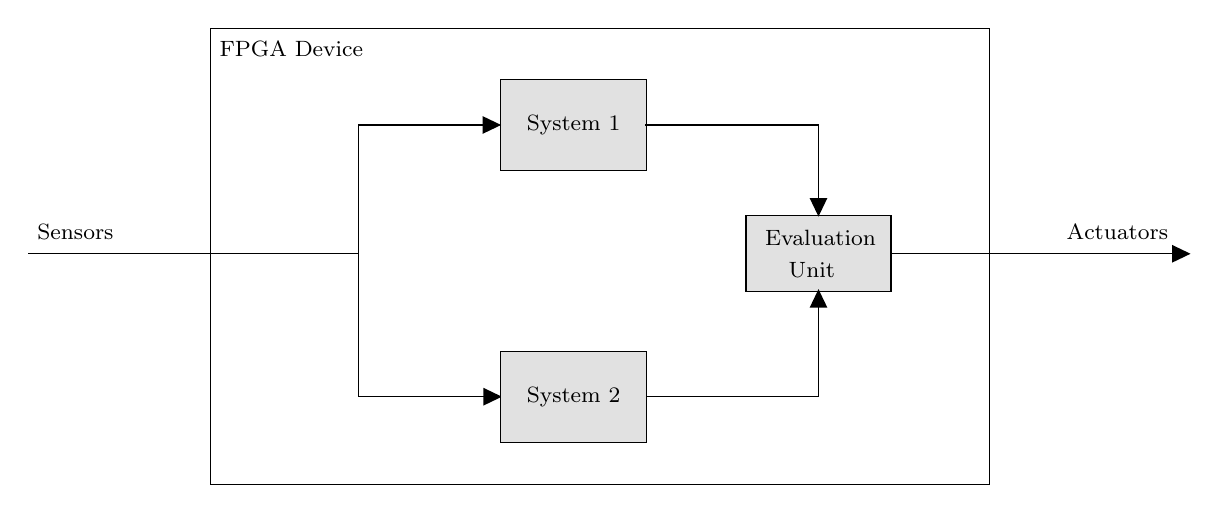
\begin{tikzpicture}[x=0.75pt,y=0.75pt,yscale=-1,xscale=1]
%uncomment if require: \path (0,300); %set diagram left start at 0, and has height of 300

%Straight Lines [id:da5881950910157023] 
\draw    (286.51,183) -- (220.3,183) ;

\draw [shift={(289.51,183)}, rotate = 180] [fill={rgb, 255:red, 0; green, 0; blue, 0 }  ][line width=0.08]  [draw opacity=0] (8.93,-4.29) -- (0,0) -- (8.93,4.29) -- cycle    ;
%Straight Lines [id:da25338917902177904] 
\draw    (220.3,52.09) -- (220.3,183) ;


%Shape: Rectangle [id:dp3450500434713657] 
\draw  [fill={rgb, 255:red, 225; green, 225; blue, 225 }  ,fill opacity=1 ] (289.05,161.14) -- (359.05,161.14) -- (359.05,204.86) -- (289.05,204.86) -- cycle ;
%Shape: Rectangle [id:dp14922514498310435] 
\draw  [fill={rgb, 255:red, 225; green, 225; blue, 225 }  ,fill opacity=1 ] (289.05,30.23) -- (359.05,30.23) -- (359.05,73.95) -- (289.05,73.95) -- cycle ;
%Straight Lines [id:da0868762150769582] 
\draw    (286.12,52.09) -- (220.3,52.09) ;

\draw [shift={(289.12,52.09)}, rotate = 180] [fill={rgb, 255:red, 0; green, 0; blue, 0 }  ][line width=0.08]  [draw opacity=0] (8.93,-4.29) -- (0,0) -- (8.93,4.29) -- cycle    ;
%Straight Lines [id:da9680613737529542] 
\draw    (220.3,114.14) -- (61.3,114.14) ;


%Shape: Rectangle [id:dp2265192536845475] 
\draw  [fill={rgb, 255:red, 225; green, 225; blue, 225 }  ,fill opacity=1 ] (407.1,95.86) -- (476.99,95.86) -- (476.99,132.42) -- (407.1,132.42) -- cycle ;
%Straight Lines [id:da668687133025897] 
\draw    (442.05,134.2) -- (442.05,183) ;

\draw [shift={(442.05,131.2)}, rotate = 90] [fill={rgb, 255:red, 0; green, 0; blue, 0 }  ][line width=0.08]  [draw opacity=0] (8.93,-4.29) -- (0,0) -- (8.93,4.29) -- cycle    ;
%Straight Lines [id:da3164126413280457] 
\draw    (442.05,93.2) -- (442.05,52.09) ;

\draw [shift={(442.05,96.2)}, rotate = 270] [fill={rgb, 255:red, 0; green, 0; blue, 0 }  ][line width=0.08]  [draw opacity=0] (8.93,-4.29) -- (0,0) -- (8.93,4.29) -- cycle    ;
%Straight Lines [id:da2018473186011438] 
\draw    (442.05,183) -- (359.3,183) ;


%Straight Lines [id:da8685031016449603] 
\draw    (442.05,52.09) -- (358.3,52.09) ;


%Straight Lines [id:da7841339318502909] 
\draw    (618.3,114.14) -- (477.3,114.14) ;

\draw [shift={(621.3,114.14)}, rotate = 180] [fill={rgb, 255:red, 0; green, 0; blue, 0 }  ][line width=0.08]  [draw opacity=0] (8.93,-4.29) -- (0,0) -- (8.93,4.29) -- cycle    ;
%Shape: Rectangle [id:dp3914738316121473] 
\draw   (149.3,5.47) -- (524.3,5.47) -- (524.3,225.2) -- (149.3,225.2) -- cycle ;

% Text Node
\draw (324.05,52.09) node  [font=\footnotesize] [align=left] {System 1};
% Text Node
\draw (324.05,183) node  [font=\footnotesize] [align=left] {System 2};
% Text Node
\draw (443.05,114.14) node  [font=\footnotesize] [align=left] {Evaluation\\ \ \ \ Unit};
% Text Node
\draw (586.05,103.64) node  [font=\footnotesize] [align=left] {Actuators};
% Text Node
\draw (84.05,103.64) node  [font=\footnotesize] [align=left] {Sensors};
% Text Node
\draw (188.05,15.59) node  [font=\footnotesize] [align=left] {FPGA Device};


\end{tikzpicture}

    \caption{FPGA (1oo2) on-chip redundancy architecture (based on diagram in \cite{Borcsok})}
    \label{onchip_redundancy}
\end{figure}

%\begin{figure}[h]
%\centering
%\includegraphics[width=0.89\textwidth]{images/SystemRedundan%cyInFPGAs.pdf}
%\caption{FPGA On-chip Redundancy 1oo2 Architecture\cite{Borcsok}}
%\label{onchip_redundancy}
%\end{figure}

%Artihmetic operations should be avoided in favour of logical operations to allow for efficient synthesis\cite{deCastro}. Transitioning algorithms and functionality requires a redesign in order to realise the benefits of an FPGA implementation\cite{deCastro}.

\section{Physical Prototype}
As part of the development of this project, a physical prototype was created. The prototype consists of a modified version of the PCB used in the microcontroller solution. In this section, the adoption of tools and components used in the implementation of the prototype are discussed. The PCB changes, made by the Socomec design team, in order to incorporate an FPGA into the existing commercial ATyS PCB are also discussed in this section. The results of the synthesis process for the design are presented. Additionally, the implemented behaviour of the prototype is presented.

\subsection{FPGA and Tool Adoption}

A number of factors need to be considered in the selection of an embedded controller. These include cost, size, performance, availability and verification capability\cite{Gomes}. The FPGA which has been adopted for the project is the Lattice Mach XO2-2000. This FPGA has 2112 LUT4 logic units. The larger package was chosen to provide as much flexibility as possible for the prototype. The MachXO2 FPGA has in-built diagnostics including configuration checks. The safety compatible version of Lattice Diamond (Lattice Diamond 2.0) was used for the development in this project. The safety standards require proven-in-use tools to be used in the development of safety-critical systems. This version of Diamond has been marked as proven-in-use by Lattice.


\subsection{PCB Re-design}

\begin{figure}[h]
\centering
\includegraphics[width=0.89\textwidth]{images/PrototypeBoard.pdf}
\caption{The prototype motor control PCB with an FPGA processor}
\label{board}
\end{figure}

The PCB was re-designed to allow for the prototyping of an FPGA solution. This PCB can be seen in Figure \ref{board}. This task was performed by design engineers at Socomec. The movement to an FPGA solution required minimal changes to the existing design. The most considerable change was the switch of the FPGA in the place of the microcontroller. Since most of the FPGA pins are freely configurable, the change from a microcontroller to an FPGA is flexible in terms of routing\cite{SalewskiSystematic}. The nature of the design implementation allowed the ADC to be implemented using a simple RC network. External memory units could be removed as the FPGA has internal memory units. A JTAG programming interface was added to the design to allow the FPGA to be reprogrammed.

\subsection{Prototyping Strategy}
\label{prototyping-strategy}
An incremental prototyping strategy was used in order to test each of the design modules independently. This involved mapping inputs to the series of push-buttons used for position acquisition and mapping the outputs to general I/O ports. This allowed the inputs of modules to be simulated and the outputs to be analysed on an oscilloscope. This provided insight into the physical behaviour of each module and allowed the design to be implemented incrementally. This process was performed after the module verification, discussed in  Section \ref{verification}. This meant that each of the individual modules had already been verified which resulted in a rapid implementation process with each of the modules working as expected. 

Despite the fact that each of the modules had been functionally verified, there were a number of problems relating to the specification which were identified while prototyping the design. For example, the naming convention was inconsistent between the schematic for the microcontroller solution and the FPGA board. This resulted in the positions being read in reverse. For example, position 1 was read as position 2. However, direction calculation and the position translation was updated and the expected behaviour was realised.

Components which were not utilised by the prototype were used as debugging interfaces. The interface used to communicate with the second control board was used to view the values produced by the ADC. This allowed the RC components to be tuned to the optimum range for the measurement voltage. It also allowed for debugging when testing the regulation control process as the values could be stepped through on the oscilloscope and the response could be analysed.

\subsection{Synthesis Results}

Mach XO2 FPGAs come in different package sizes for which the number of logic units and the number of pins varies as well as the cost. The synthesised prototype design used 36\% of the capacity of the Mach XO2-2000 FPGA used in the project. This leaves 1352 of the 2112 logic units in the FPGA available for use. This additional space could be used for the diagnostic components and redundancy architectures discussed in Section \ref{diagnostic-section}. Alternatively, the package size could be reduced. The design used 20 of the
100 FPGA I/O ports. This was composed of eight for the position measurement, three for the command input, three for each of the ADC measurements and six for the motor control signals.

\subsection{Prototype Behaviour}
The prototype successfully implemented the safety function of the device. Physical prototyping allowed for the behaviour of the designed system to be verified and compared against the existing solution. Functionality of the physical prototype includes performing the core safety function of the device, performing a transfer from one power source to another. This behaviour requires the correct acquisition of commands and position and calculation  of the required movement as well as the translation of this into a control sequence to drive the motor. Additional functionality includes the regulation of the current in order to control the response in cases of stalled or blocked motors. The timeout and movement retry behaviour in the microcontroller solution was also replicated in the design and prototype.

\section{Design Conclusion}

The FPGA-based system was designed based on the original microcontroller-based system specification. The motor control behaviour was identified as the safety function of the device. The requirements that allow this to be performed were derived from this specification and became the requirements for the design of the FPGA system. Following the V-model process, a system architecture was derived from these requirements. Four main system processes were identified in order to meet the requirements and were integrated as modules to form the system architecture. These modules are Input Processing, ADC, PWM Regulation and Motor Driving. The design and implementation of these modules has been described in this section. Additionally, the clock design was discussed. The planning of diagnostics was also presented; however, the implementation of these diagnostics was outside the scope of the project. Finally, the physical prototype which was created as part of the development in this project was presented in this section. The prototype successfully replicated the safety function behaviour of the microcontroller board in the ATyS.
\chapter{Verification}
\label{verification}

This section describes the verification activities undertaken as part of this project, giving examples of how they were applied to each of the modules in the design. Firstly, the use of the V-model process for verification in this project is discussed. This is followed by a discussion of how verification methodologies were utilised throughout verification, simulation and testing in this project. The verification plan, which maps directly to the original project requirements, is presented. The verification results are then presented. The verification of each module in the system architecture is discussed with example simulation and verification results. 

In the interest of maintaining clarity of terminology used in this context, terms will be explained. In this section, verification will refer to the direct mapping and confirmation of functionality to the requirements of the system. Simulation will comprise of the analysis of produced waveforms. Testing will cover activities that incorporating timings to ensure the correct physical behaviour of the design. The term Modules will be used to refer to the high level system modules in the system architecture. There are four modules in the design: Input Processing, PWM Regulation, ADC and Motor Driving. Sub-modules will be used to refer to any design unit used within the high-level module. These sub-modules directly map to an individual requirement whereas the modules refer to a group of requirements.

\section{Verification Stages}

The V-model, shown in Figure \ref{V-model}, encourages verification of every level of the design. The verification stages follow a bottom-up methodology with a complimentary verification stage for each design activity. The first stage involves post-layout simulation to check the conformity of the design to the design rules set by the FPGA. This activity is performed automatically by the Lattice Diamond tool-suite. Following this, individual modules are verified. This stage benefits from small contained modules with a single testable functionality. After the modules have been verified, the integration of and interactions between the modules can be verified. This process can be repeated until all modules are integrated, at which point the complete design is verified. Direct validation of requirements is the final verification stage in the V-model. Each of the requirements of the design must be validated in order to produce a validated VHDL design.

Requirements at each phase must be directly testable in order to produce a validated design. During the design phases, a test plan was produced in order to verify the requirements of that phase. This includes behavioural verification which involves ensuring the outputs produced by the unit under test correspond correctly to the input sequence. Using VHDL, it is also possible to accurately model the timing behaviour. This makes it easier to verify the real-time behaviour required by motor control applications.

%In order to test analogue components, mixed-signal simulation tools can be used\cite{Acero}. 

\section{Verification Methodologies}

Verification methodologies were adopted to aid the automation of verification, simulation and testing in this project. Two methodologies, introduced in Section \ref{litreview}, were adopted in order to perform the required verification for this project: UVVM (Universal VHDL Verification Methodology)\cite{uvvmref} and OSVVM (Open Source VHDL Verification Methodology)\cite{osvvmref}. UVVM has been adopted in order to provide stimulus and value checking whereas OSVVM has been adopted to provide automatic coverage collection. The application of these methodologies is described below.

\subsection{Universal VHDL Verification Methodology}

UVVM was applied to the design for simulation stimulus, value checking and timing verification. A number of functions are provided by the methodology for analysing the values of signals at different points in a simulation which can be triggered by events or time-windows. This allows the behavioural response of the design to be verified alongside the timing of the response. As well as producing graphical simulation results which display the states of each signal in the unit under test (UUT), textual results can be produced to automate the checking of required values at different points in the simulation. The use of these functions allowed the functional and timing behaviour of the system modules to be verified.

Figure \ref{position_uvvm} shows the application of UVVM to an example design module, the Position Acquisition module. The diagram, generated by the VHDL editor Sigasi, shows how the inputs of a UUT can be stimulated and how its outputs are monitored by the UVVM process (labelled uvvm\_driver in the diagram). This is shown in Figure \ref{position_uvvm}. The diagram shows the input clock, reset and position buttons being provided to the left of the UUT by the UVVM driver. This process allowed each of the test cases to be applied to the UUT. The response of the calculated position, shown on the right of the UUT, was then compared to the expected position for each case. This methodology was used for each module in the design. Example UVVM code used to verify the Position module is shown in Appendix Item \ref{UVVM_Position_Code}.

\begin{figure}[h]
\centering
\includegraphics[width=0.75\textwidth]{images/uvvmblockdiagram.pdf}
\caption{UVVM simulation setup showing the input driving and output sensing for the Position Acquisition module of the ATyS design (diagram generated by Sigasi from the design code of the project)}
\label{position_uvvm}
\end{figure}



\subsection{Open Source VHDL Verification Methodology}

The application of OSVVM allowed for the 100\% coverage, required by SIL, to be proven automatically. Functional coverage was applied to the design to ensure that the test plan had been completed. By setting up transition bins, the states of the UUT were tracked throughout the simulations and a calculation of the coverage was performed by the OSVVM process. Example OSVVM code, showing the mapping of state machine transitions for the example UUT is shown in Appendix Item \ref{OSVVM_Motor_Bins}. The operation of this tracking can be seen in Figure \ref{osvvm_sim} where the OSVVM coverage process monitors the UUT throughout the simulation. This diagram, also generated using Sigasi, shows how the OSVVM process monitors the stimulus provided by the UVVM process as well as the states of the example UUT. This was applied to all state machines in the design to ensure that all valid states of the system were realised in the simulation process.

\begin{figure}[h]
\centering
\includegraphics[width=\textwidth]{images/osvvmblockdiagram.pdf}
\caption{OSVVM process tracking the coverage on a UVVM driven simulation (diagram generated by Sigasi from the design code of the project)}
\label{osvvm_sim}
\end{figure}

\section{Verification of Requirements}

In accordance with the V-model, the project requirements were directly mapped into the verification plan. This was to ensure a fully validated design. The requirements table (Table \ref{requirements-table}) in the Design section shows each of the project requirements. It is divided into requirements for each of the four modules of the system architecture. The requirements displayed in this table have been mapped directly into the verification plan shown in Table \ref{requirements-verification-table}. It shows the requirement identifier, a description of the tests carried out and a summary of the results for each module requirement. The verification results for each module are presented in the following sections.

\begin{table}[tH]
\centering
\begin{tabular}{ |p{0.15\textwidth}|p{0.4\textwidth}|p{0.4\textwidth}| }
 \hline
 \multicolumn{3}{|c|}{ATyS Motor Control Verification Table} \\
 \hline
 Requirement & Description & Verification Results \\
 \hline
 \hline

 Input R1 & Provide all possible input combinations and compare the results with a look-up-table & A sweep through all command inputs was done and the translation was verified against the original specification \\
 \hline 
 Input R2 & Provide all possible input combinations and compare the results with a look-up-table & Each position was input and the translation was verified against the specification (see Figure \ref{position_sim})  \\
 \hline 
 Input R3 & Check all 27 combinations of position and command and verify the correct movement is taken & Each combination produced the correct direction and control signals \\
 \hline 
 Input R4 & Run through each of the possible control stages and ensure the correct timings and values of processes & Timings and control signals match the specification \\
 \hline
 PWM R1 & Check the duty-cycle output for a motor movement over each of the defined stages & The duty-cycle value produced in each of the stages was verified against the specification \\
 \hline
 PWM R2 & Model a stalled motor in simulation (motor resistance measured to be \si{47}{\ohm}) and ensure regulation around the correct current value & The simulation model allowed the regulation process to be fine-tuned and it settled on an accurate value (see Figure \ref{regulation_sim}) \\
 \hline 
 PWM R3 & Check the frequency and duty-cycle of the output against the specified input duty-cycle value & A range of different duty-cycles were provided to the generator and the output was verified to match exactly \\
 \hline 
 PWM R4 & Verify that the current flag is raised half-way through the generation process & A range of different duty-cycles were input and each produced a flag exactly in the middle of the on-time \\
 \hline
 PWM R5 & Input the range of valid voltages (150V - 333V) and verify that the output matches the formula & A sweep of the input values obtained a response which matched the specification \\
 \hline
 ADC R1 & Model the RC input and supply an analogue value and verify the digital output & ADC accurately simulated for a sawtooth input (see Figure \ref{adc_sim}) \\
 \hline
 ADC R2 & Model the RC input and supply an analogue value and verify the digital output & ADC accurately simulated for a sawtooth input (see Figure \ref{adc_sim})\\
 \hline
 Drive R1 & Verify that the correct IGBT is driven for each direction (see Figure \ref{motor_control_circuit} which shows the required IGBT signals for each movement) & The motor control process was simulated and the IGBT stimulus was verified against the expected signals (see Figure \ref{igbt_sim})\\
  \hline
 Drive R2 & Verify that the correct Thyristor is driven for each direction (Figure \ref{motor_control_circuit} shows the required Thyristor signals for each movement) & The motor control process was simulated and the Thyristor stimulus was verified against the expected signals \\
 \hline
\end{tabular}
\caption{Verification table for the ATyS motor control requirements}
\label{requirements-verification-table}
\end {table}

\subsection{Input Processing Verification}

The primary input stage of the design, the Input Processing Module, comprised of a number of sub-modules; each of which were verified in isolation. First of all, the response to different position readings was verified against the specification. The simulation results for the Position sub-module are shown as an example in Figure \ref{position_sim}. The simulation shows the buttons on the bottom eight rows, which were stimulated using UVVM, going through each valid combination. The value for the position is then calculated. It can be seen visually that the calculated position (output\_position\_s) is exactly the same value as the stimulated test case (position\_in\_s). The simulation also displays the behaviour of intermediate signals (buttons\_read\_in\_s). The numbers in the simulation do not correspond to the actual position due to the position encoding scheme, for example, Position one is represented by a number three in the encoding scheme. The translation logic can be seen in Appendix Item \ref{position-multiplexing-code}.

\begin{figure}[h]
\centering
\fbox{\includegraphics[width=\textwidth]{images/Position-sim.pdf}}
\caption{Simulation of the Position Acquisition module for each input combination (requirement: Input R2)}
\label{position_sim}
\end{figure}


In addition to the simulation results for each module, value checking was also applied to the design using UVVM to ensure the correct value is calculated. The results of the UVVM checking for the Position sub-module are shown in Figure \ref{uvvm_results}. The textual output corresponds to the same simulation displayed for the Position sub-module. As the simulation progresses, the values at any time along the simulation can be verified and the results are summarised at the end of the simulation. If a value is found to be incorrect for any of the checks then it is flagged and the actual value is presented which aids debugging. The textual response for this module shows each of the stages of the verification plan. The module was swept through from Position one, through each intermediate position, to Position two. Example UVVM code for a single check, which corresponds to a line in the summary table, is shown in Appendix Item \ref{UVVM_Position_Code}. The code shows the stimulation, value checking and timing verification that are applied using UVVM methods. This pattern was applied for each position in the simulation.
The results were also checked for invalid position inputs. Timing verification, ensuring the filter is working as expected, is also performed and the results are presented.

\begin{figure}[h]
\centering
\fbox{\includegraphics[width=\textwidth]{images/uvvm_results.png}}
\caption{UVVM verification output example for the Position module simulation}
\label{uvvm_results}
\end{figure}

The other sub-modules in the Input Processing module were also simulated and verified. The same process that was applied to the Position Acquisition sub-module was applied in the verification of Command interpretation. Each of the valid commands were swept through and the output of the Command sub-module was monitored and verified using UVVM. The other sub-modules in the Input module relate to the control of direction and timings of the movement. For the verification of the sub-module for requirement Input R3, responsible for the decision making in terms of movement and direction, each combination of command input and position was provided and the expected result was analysed. The response included raising a flag to indicate that movement is necessary and providing the correct direction of movement. The sub-module which was responsible for the timing control of the motor control process was verified using UVVM timing functions. The UVVM functions wait for a given event and then can verify that the timing of that event matches the required time. Alternatively, they can wait a given time and verify that the value is correct at that time. This was applied over several of the application cases including a successful movement first time, a successful movement upon a retry and an unsuccessful movement in order to verify that the response of the design matched the specification for each case.

\subsection{ADC Verification}

In order to verify the ADC, an analogue input must be modelled by the simulation. This required creating a model of the RC input stage. The ADC, which was obtained from Lattice, came with a verification file. In this verification file, integrators are used to simulate the RC input stage and the comparitor at the input of the FPGA. A saw-tooth input was generated in this simulation in order to verify the response of the ADC. 

\begin{figure}[h]
\centering
\fbox{\includegraphics[width=\textwidth]{images/ADC-sim.pdf}}
\caption{ADC simulated response to a saw-tooth waveform (requirements: ADC R1 and ADC R2)}
\label{adc_sim}
\end{figure}

The simulation results in Figure \ref{adc_sim} show the response of the ADC to this saw-tooth input. The response can be seen to follow the saw-tooth ramp closely. When the saw-tooth resets and falls from the maximum value to the minimum value, the ADC can be seen to follow the value with the behaviour of an averager as it falls through an intermediate value before increasing again. UVVM was applied to this simulation throughout to ensure the value is within a one-bit tolerance of the input value for each reading. The ADC produces periodic values and holds the value until it has calculated the next one so the response is more stepped than the simulated analogue input. 

\subsection{PWM Regulation Verification}
\label{regulation-results}
In order to test the PWM regulation scheme, the regulation loop, shown in Figure \ref{motor_control_loop}, must be simulated. This includes modelling the motor in order to verify the response to an actual motor. Under normal switching conditions, regulation of motor current is not needed as the current is consistently below 1.5A. The regulation process operates when the motor is stalled or blocked. In order to verify the response of the motor to these conditions, a stalled motor has to be modelled in the simulation. It is difficult to accurately simulate the actual response of an analogue motor controlled by a VHDL design\cite{Dubey}. Matlab can be used for mixed-signal simulations\cite{Dubey}, however; it will not be adopted by this project as a simplified model of the stalled motor was sufficient for regulation testing and fine-tuning. The model consisted of a VIR calculation based on the PWM signal (V), the resistance of the motor (R) and the calculated resulting current (I) which was fed back into the regulation unit. UVVM was used to perform the calculations required to model the motor and provide the new stimulus.

\begin{figure}[h]
\centering
\fbox{\includegraphics[width=0.65\textwidth]{images/Regulation-sim.pdf}}
\caption{PWM regulation simulation of a stalled motor modelled in UVVM (requirement: PWM R2)}
\label{regulation_sim}
\end{figure}

The simulation results for the PWM Regulation module are shown in Figure \ref{regulation_sim}. The diagram shows the response of the duty-cycle to the measured current for the regulation process. The regulation module aims to keep the current value at a nominal value. It achieves this by adjusting the PWM duty-cycle, which drives the motor, based on the measured current from the ADC. In this simulation, the current is calculated from the effect of the duty-cycle value on a fixed resistance. It can be seen in the diagram that the initial value of current is measured to be too low, compared to the regulation value. In response to this, the regulation module increases the duty-cycle. The response of the motor model produces a current which is now above the regulation value, the duty-cycle is then reduced accordingly. This process repeats until the values stabilise and the regulation current is achieved. In this example, the regulation current was set to the ADC value of 155 and the value alternates between 155 and 156. The response, which can be seen in this simulation, is typical to that of a proportional controller. UVVM checking was also applied to ensure that each of the PWM Regulation requirements were met by the design. The additional sub-modules which were responsible for providing the correct control signals to the regulation process were generated using UVVM for this simulation and were verified separately.

The PWM module design contains a number of state machines in order to generate the required control signals; each of which needs to be fully verified. OSVVM was applied to each of them to ensure that each machine reaches each possible state during the simulation. The application of state transition monitors provides instant and automatic feedback. An example response from OSVVM, applied to the PWM control state machine, can be seen in Figure \ref{osvvm_results}. The response shows a calculation of the state coverage. In this case the coverage is 100\%. The results for each transition are printed in the response. This includes a count of the number of transitions between states throughout the simulation for each mapping and a flag indicating that the transition occurred. The OSVVM code which set up these transition bins can be seen in Appendix Item \ref{OSVVM_Motor_Bins}. This instant feedback ensures that the test plan has been completed by ensuring that all states are realised in the simulation. OSVVM was applied to all state machines in the design and identified cases which were not originally covered in the test plan. The test plan was modified in iterative cycles and the final test-suite provided 100\% state coverage.

\begin{figure}[h]
\centering
\fbox{\includegraphics[width=\textwidth]{images/osvvm_results.png}}
\caption{OSVVM state coverage results for the PWM control state machine (requirement: PWM R1)}
\label{osvvm_results}
\end{figure}

\subsection{Motor Driving Verification}

The Motor Driving module is required to drive the correct IGBT and Thyristor combinations based on control signals provided by other modules. The behavioural response to each of the control signal combinations must be verified against the specification to ensure that it is not possible for invalid combinations of IGBTs and Thyristors to be driven. The output control signal combinations from the Input Processing and PWM Regulation modules were generated using UVVM and the response was verified using the same methodology.

The simulation results for the IGBTs during a motor movement can be seen in Figure \ref{igbt_sim}. The control signals which were created as part of the motor control process were simulated. The conditions for each respective IGBT being driven are checked by the simulation. The PWM signal, produced by the simulation to model the accurate behaviour of the system, was sent to the IGBT for the correct direction indicated. For example, the simulation shows the completion of one of the sub-module requirements for the IGBT: if the IGBT is enabled (en\_db\_o\_s is set to 1) then the PWM generated by the regulation process (pwm\_i\_s) should be passed directly to the IGBT for the given direction (pwm\_db\_o\_s). Each of the combinations of the control signals was verified using UVVM. The braking phase can also be seen in the diagram where the brake\_i\_s signal is driven. For this phase, which is required to stop the motor, each of the IGBTs are driven. 

\begin{figure}[h]
\centering
\fbox{\includegraphics[width=\textwidth]{images/IGBT-sim.pdf}}
\caption{Simulation of the IGBT throughout the simulated motor control process (requirement: Drive R1)}
\label{igbt_sim}
\end{figure}



\section{Further Verification}
Behavioural verification of each module of the design was performed using UVVM; however, there were some verification activities, required by SIL, which were not completed in simulation for this project. These activities include system-level verification which is related to the interaction between different modules. Additionally, gate-level simulations which give insight into the synthesised timings of the design were not performed using UVVM.

\subsection{System Verification}

System behaviour can be validated by verifying multiple modules and their interactions. For this project, this process was done on the physical prototype. As described in the prototype creation Section \ref{prototyping-strategy}, the modules were tested on the PCB by incrementally integrating sub-modules. By verifying this using UVVM the benefits of automatic verification could be realised. This would provide the design with a more comprehensive test-suite which verifies each level of the module. Any number of modules can be incorporated into a simulation for UVVM. This could scale up to the entire design where the requirements of the entire end-to-end system can be validated. This is the final process of the V-model. 

\subsection{Gate-level Simulations}

Gate-level simulations can be performed on the synthesised design. This allows accurate modelling of the timing behaviour of the system. Where register-transfer-level simulations provide behavioural verification, gate-level simulations provide insights into true time-based behaviour. Behavioural verification was the focus for this project. The prototyping activities on the physical PCB gave insight into and verification of the general timing behaviour of the system; however, by applying verification methodologies to the gate-level design, the timing verification of the design could be realised. 



%Others:
%How OSVVM is being used for this
%SIL requires 100\% coverage
%How UVVM is being used for stimulation
%Simplifies the verification code and makes it easier to read/understand
%How UVVM is being used for value checking
%Automates the validation process (prevents manual inspection of simulation results, reduces the verification time)
%Using UVVM for timing analysis
%Essential for the verification of time-based requirements (real-time systems) like motor control (find source)
%Automates the validation process



% realtime digital simulator for motor drives? \cite{Zhang}
% VHDL-AMS (mixed signal) \cite{Acero}


\section{Verification Conclusion}

Verification methodologies were systematically applied to directly verify the project requirements. UVVM was used to verify the functional behaviour of each modules in the design to ensure that they matched the specification. The automated value checking of UVVM reduced the need for manual inspection of simulation graphs and allowed for instant verification feedback. OSVVM was applied to each of the state machines in the system to ensure that they were all fully covered by the simulation. OSVVM was applied to map each of the transitions of state machines in the design to provide coverage metrics for the simulations. The verification of the design validated all of the project requirements with a 100\% state coverage. System and gate-level simulations were applied on the physical prototype of the project. By applying UVVM to these verification areas, the benefits of methodologies could be realised for integration and timing behaviour. All of the modules in the design were verified individually and each of the requirements were directly mapped into the verification plan providing a comprehensive coverage of validation of the requirements of the design.  
\chapter{Results}
\label{results}

The behaviour of the alternative FPGA solution needs to accurately replicate the behaviour of the existing microcontroller solution. There are two behavioural processes which were implemented by the prototype: the behaviour for a successful movement from one position to another and the regulation process which limits the current. The first of these scenarios occurs during normal operation to transfer the connection from one power supply to another. The regulation process must be used to limit the motor current in the event of a stalled or blocked motor. As part of the results for this project, the behavioural response to each of these scenarios is compared. 
The motor control function is compared between the two solutions in Section \ref{atys-movement}. The response of the current regulation process is compared in Section \ref{current-reg}. 

The motor control process output is a PWM signal of a duty-cycle which is calculated and generated by the ATyS processor. This duty-cycle value is compared for each of the solutions as part of the results. Additionally, the motor current is also displayed and compared which represents the response of the motor. For each of these tests, the data was taken directly from the Oscilloscope. One million points were taken over five seconds for each reading. The duty-cycle calculations were performed in Excel using the times between the rise and fall of the supplied signal.

\section{Experimental Setup}

\begin{figure}[h]
\centering
\includegraphics[width=\textwidth]{images/AtysExperimentalSetup.jpg}
\caption{The experimental setup for the FPGA vs microcontroller comparisons}
\label{atys_experimental_setup}
\end{figure}

The experimental setup for each of the tests can be seen in Figure \ref{atys_experimental_setup}. The equipment used for this experiment included an AC power supply, an oscilloscope, an ATyS casing and an ATyS command interface. Each of the PCB solutions being compared were placed into the same model of ATyS casing for experimentation. The oscilloscope had two inputs for each of the experiments: the motor current which was measured from the connection between the rotor and the stator, and the voltage supply to the IGBTs which was measured directly on the PCB. The supply voltage was set to 250V for the motor movement test and was reduced to 200V for testing the regulation processes. The same model of motor was used for both the FPGA and microcontroller boards. For the stalled motor test, the rotor from one motor was connected to the stator of the other to prevent any movement.
The same ATyS switch, the load for the motor, was used for each set of results. 

\section{ATyS Movement Test}
\label{atys-movement}

The core functionality which had to be replicated by the design in this project is the motor control of the ATyS system. This safety function allows the power supply connection to be transferred. The first test will be a comparison between how each of the processors, microcontroller and FPGA, perform this core activity. 

As described in the design section, the motor control processes follow a number of defined phases which determine the PWM provided to the motor. 
The motor control contains five discrete phases: PWM startup, PWM minimum, PWM increase, PWM regulation and braking. These phases are represented as states in a state machine in the FPGA design code which is shown in Appendix Item \ref{pwm-state-machine-code}. The stimulation of the motor during the control process has been defined for previous iterations of the ATyS device. An initial startup phase is used in order to activate the IGBTs and Thyristors required. The PWM, which supplies the IGBTs, is then set to the minimum for a short period before being increased to the maximum calculated value. This value is held until the required motor position is reached. At this point, braking is applied to each of the IGBTs. The results of the test, which involved the movement from position one to position two, are shown in Figure \ref{movement_test}.

\begin{figure}
\centering
\begin{subfigure}{0.8\textwidth}
\centering
\begin{tikzpicture}
%\pgfplotsset{scale only axis, scaled x ticks=base 10:3, xmin=0, xmax=0.06}

% current
\begin{axis}[
    %legend pos=south west,
  legend style={at={(0.5,0.03)},anchor=south},
  axis y line*=right,
  axis x line=none,
  ymin=-2, ymax=2,
  ylabel=Motor Current (A)
]

\addlegendimage{/pgfplots/refstyle=Duty_Cycle}\addlegendentry{Duty-cycle}
\addplot[red!60]table {Graphs/MicroMovement/MotorCurrent.txt};
\addlegendentry{Motor Current}
\label{Motor_Current}
\end{axis}

% pwm
\begin{axis}[
axis y line*=left,
ymin=-10, ymax=110,
xlabel=Time (s),
ylabel=PWM Duty-cycle (\%),
]
\addplot[blue!80]table {Graphs/MicroMovement/DutyCycle.txt};
\label{Duty_Cycle}
\end{axis}


\end{tikzpicture}

\subcaption{Micro-controller Motor Control}
\label{MICROgraph}
\end{subfigure}

\input{Graphs/FPGAMovement/FPGAMove.tex}
\caption{Graphs showing the motor response to the control sequence applied by the microcontroller (\subref{MICROgraph}) and FPGA (\subref{FPGAgraph}) for a successful movement}
\label{movement_test}
\end{figure}

The microcontroller motor control process starts with a preset startup phase which involves the transistors activation before the duty-cycle is reduced to 20\%. This is followed by increasing of the PWM duty-cycle gradually to the maximum value. The maximum value is calculated based on the value of the supply voltage. In this experiment, the maximum PWM was calculated to be 75\%. When the maximum value is reached then the regulation phase is triggered. However, under normal conditions and the conditions for this test, the motor current never increases above the regulation value of 1A and so no regulation is performed. Therefore, throughout this phase, the duty-cycle is held constant. This phase ends when the correct motor position is reached. Upon reaching the position, the braking phase is triggered in which both IGBTs are driven full. This causes a spike in the current in order to stop the motor.

In the graph showing the response from the FPGA system to a motor movement, the same stages of motor control can be seen. It starts with an activation spike in duty-cycle. The PWM then drops to the same minimum value of 20\%. The ``increase phase'' is done over a longer time in the FPGA. This is due to the settings in the control algorithm. The maximum value, for the same voltage, was calculated at 80\% and so this was the constant duty-cycle value for the regulation stage. The same current spike can be seen in the FPGA solution.

The same stages can be seen in each of the designs. Some of the calculation details in the FPGA solution differ slightly. For example, the maximum PWM calculation and the slope of the PWM increase. The current response is similar in each motor control process. The current follows an initial peak in the increase phase and then stabilises at around 0.5A before spiking at the braking phase of the control.

Overall, the current response for the microcontroller and FPGA solutions are almost identical. They follow the same distinct phases. Some of these phases differ slightly as the calculation of different values, for example, the maximum PWM differs. The rate at which the PWM increases is slower in the FPGA. This could be updated in the control algorithm calculation to obtain the same response.

\section{Stalled Motor Test}
\label{current-reg}
If the motor of the ATyS is blocked then the current can spike to very high values. The current therefore needs to be regulated to prevent these damaging high currents. In order to test this behaviour, a stalled motor was used. This was achieved by connecting the rotor of one motor to the stater of the other. With the exception of switching the motor for a stalled version, the setup is the same as for the previous test and can be seen in Figure \ref{atys_experimental_setup}. For this test, the supply voltage was set to 200V. This means the calculation of the maximum PWM is different when compared to the motor movement tests.

The regulation process is intended to regulate the current around 1A. The device works in AC and so there will be 50Hz variations but these should be contained by the process. The response of the microcontroller to these conditions can be seen in Figure \ref{stalled_motor_test}\subref{MICROREGgraph} and the FPGA response can be seen in Figure \ref{stalled_motor_test}\subref{FPGAreggraph}. In these graphs, the PWM Duty-cycle produced by the processor, which drives one of the IGBTs, is graphed in blue against time. This allows the regulation process, and it's effect the duty-cycle, to be visualised. The motor current, shown in red, allows for the effect of the regulation process to be seen.

\begin{figure}
\centering
\input{Graphs/MicroRegulation/MicroRegulation.tex}
\begin{subfigure}{0.8\textwidth}
\centering
\begin{tikzpicture}
%\pgfplotsset{scale only axis, scaled x ticks=base 10:3, xmin=0, xmax=0.06}

% current
\begin{axis}[
    %legend pos=south west,
  legend style={at={(0.97,0.97)},anchor=north east},
  axis y line*=right,
  axis x line=none,
  ymin=0, ymax=4,
  ylabel=Motor Current (A)
]

\addlegendimage{/pgfplots/refstyle=Duty_Cycle}\addlegendentry{Duty-cycle}
\addplot[red!60]table {Graphs/FPGARegulation/FPGARegulationCurrent.txt};
\addlegendentry{Motor Current}
\label{Motor_Current}
\end{axis}

% pwm
\begin{axis}[
axis y line*=left,
ymin=-10, ymax=110,
xlabel=Time (s),
ylabel=PWM Duty-cycle (\%),
]
\addplot[blue!80]table {Graphs/FPGARegulation/FPGARegulationDC.txt};
\label{Duty_Cycle}
\end{axis}

\end{tikzpicture}

\subcaption{FPGA Current Regulation}
\label{FPGAreggraph}
\end{subfigure}

\caption{Graphs showing current regulation process in the microcontroller (\subref{MICROREGgraph}) and FPGA (\subref{FPGAreggraph}) by applying the control process to a stalled motor}
\label{stalled_motor_test}
\end{figure}

The microcontroller response initially follows a preset startup phase. This is the same as the process for the first test as no regulation is done in this phase. The regulation phase is triggered by the reaching of the maximum PWM value which is calculated by the regulation process. When this phase is complete, the motor current is higher than 1A, around 3A, and so the system reacts and drops the duty-cycle of the PWM to 35\% which reduces the power being supplied to the motor. The current reduces due to this action and so the PWM duty-cycle increases in response. The behaviour of a proportional controller can be seen. It continues to overshoot before settling on a value of around 50\% duty-cycle. The current regulates consistently around 1A with some periodic variations.

The FPGA response also starts with the preset startup phase which increases the current over the desired limit. Once the regulation process starts, the duty-cycle is reduced dramatically to 20\%. The duty-cycle is then increased in response. The value then toggles between 40\% and 50\% in order to regulate the current. The current response regulates consistently around 1A throughout the regulation phase.

For this test, the regulation process of each of the processors is being compared. Each of the regulation processes drops the duty-cycle in response to the initially high current. The motor current for each of the solutions is around 3A after the preset startup phase. The current response to the drop in duty-cycle, performed by each of the processors, is the same. After the initial response, the microcontroller acts as a proportional controller and both the duty-cycle and the current settle around a value after a few overshoots in the regulation process. In the FPGA, the behaviour after the initial drop is slightly different. The value increases and begins to regulate around 1A more quickly and without any overshoot. 

Once the values begin to regulate, the processes are slightly different. Each of the solutions regulates the current successfully between 0.5A and 1.5A. In the microcontroller, periodic variation is seen in the duty-cycle but it remains fairly constant. The variations that do occur can be seen to correspond to variations in the motor current. In the FPGA, the duty-cycle varies more throughout the regulation process. The device toggles the response continually between 40\% and 50\% in response to the 50Hz fluctuations. The response of the current to this regulation process is much smoother than in the microcontroller solution.  

Overall, the current response of the two systems to a stalled motor is almost identical (see Figure \ref{stalled_motor_test}). In these conditions, spikes in current could be dangerous and so the current must be regulated. The FPGA regulation process was modelled from the existing microcontroller and so the similarities and differences have been compared as part of this test. It was found that, although the regulation processes differ, the current response is almost identical. The FPGA reaches the regulation value, 1A, quicker than in the microcontroller process. Additionally, the current variations present in the microcontroller solution are eradicated in the FPGA solution.

%\section{ADC Testing}



%\begin{figure}[h]
%\centering
%\begin{tikzpicture}
%\pgfplotsset{scale only axis, scaled x ticks=base 10:3, xmin=0, xmax=0.06}

% current
\begin{axis}[
    %legend pos=south west,
  legend style={at={(0.97,0.03)},anchor=south east},
  %axis y line*=left,
  %axis x line=none,
  ymin=0, ymax=2,
  xlabel=Time (s),
  ylabel=Voltage (V)
]


\addlegendimage{/pgfplots/refstyle=adc_results_graph_vin}
\addlegendentry{${V_{in}}$}
\addlegendimage{/pgfplots/refstyle=adc_results_graph_adc}
\addlegendentry{${V_{out}}\ ADC$}
\addplot[red!60]table {Graphs/ADCResults/ADC_Vin.txt};
\label{adc_results_graph_vin}
\addplot[blue!80]table {Graphs/ADCResults/ADC_Vadc.txt};
\label{adc_results_graph_adc}
\end{axis}



\end{tikzpicture}

\label{FPGAgraph}
%\caption{ADC response to a saw-tooth voltage input}
%\label{adc_results}
%\end{figure}

%% simulation results
%\begin{figure}[h]
%\centering
%\input{Graphs/ADCSimulation/ADCSimGraph.tex}
%\caption{ADC simulation showing response to a saw-tooth voltage input}
%\label{adc_simulation}
%\end{figure}

\section{Results Conclusion}

The behaviour for both a successful and an unsuccessful motor movement has been replicated successfully in the FPGA solution. The current response to a successful movement is almost identical for the microcontroller and the FPGA. The device successfully performs the movement with the same process stages as the microcontroller system. The current regulation scheme, despite slight differences in behaviour, is also well matched. The current regulation in the FPGA solution reaches the regulation value faster than in the microcontroller and is a much smoother regulation.
\chapter{Evaluation}
\label{evaluation}

In this section, the results of the project will be evaluated against the initial aims and objectives set out in Section \ref{introduction}. The overall aim of the project was to enhance the functional safety of the ATyS device through the design and development of an FPGA-based system. This was to be done by following the standardised safety integrity level (SIL) framework. The extent to which this overarching aim was achieved is discussed below in Section \ref{evaluation-of-aims}. Using the SIL framework, the functional safety of the device will be discussed. A number of objectives were laid out in the introduction in order to achieve this aim. The extent to which these objectives were achieved is discussed below in Section \ref{evaluation-of-objectives} along with a suggestion of how they can be built upon in the future.


\section{Evaluation of Project Aims}
\label{evaluation-of-aims}
The overarching aim for the project was to investigate the advantages of an FPGA-based ATyS processor solution with a focus on the functional safety. Safety certification is a process of verification that the system developed follows the relevant SIL guidelines. In this section, the evaluation of the achievement of this aim will relate to how closely these guidelines were followed throughout the development phases of the FPGA-based ATyS prototype. An implicit aim of the project was to replicate the safety-related behaviour of the existing microcontroller solution. 

\subsection{Safety Integrity Level Evaluation}

As described above, the SIL framework standardises the claim of functional safety of a device application and there are two sets of processes which need to be followed to achieve this\cite{IEC61508}. The first of which is related to the prevention of systematic errors through following the recommended processes. The second set of processes are concerned with the detection and correction of online errors. Each of these sets of processes must be followed in order to claim a safety integrity level. The success in achieving each of these is discussed in this section.

%\subsection{Prevention of Systematic Errors}
The recommended V-model development process was followed closely throughout the design of the FPGA-based system. The logical flow from safety requirements elicitation through derivation of system architecture and down to the module implementation was performed in this project and is described in the design section. The initial verification phases of the process were followed throughout this project. Each module was functionally verified against its requirements. System-level verification was conducted on the physical prototype built as part of the project. The overall validation phases of the V-model were also performed on the physical prototype rather than in an automated test-bench. This allowed the behaviour to be compared with the existing solution.

The V-model was a powerful tool in driving the development in the project. As well as encouraging verification throughout development, the V-model process required the understanding of project requirements before proceeding with the design. This was especially important because of the nature of this project. The safety requirements, which were derived from the system requirements, had to be well understood in order to contain the scope of the prototype and focus on safety-related aspects of the design, rather than a straight functional migration from microcontroller to FPGA.



%\subsection{Diagnostics}
Diagnostic measures were planned as part of this project. As discussed above, redundancy architectures and on-line verification components can be added to FPGA designs without impairing the performance\cite{Dubey}. These diagnostics, which are required by the standards in order to detect and control errors, were not implemented as part of this project and form part of the identified further work (see Section \ref{evaluation-of-objectives} below).


Overall, the foundations for claiming a SIL for this device application have been laid through the adoption of recommended processes. With the completion of a number of additional activities, such as gate-level and system-level verification and the addition of diagnostic components, a safety integrity level could be claimed\cite{IEC61508}.

\subsection{Microcontroller Behaviour Execution Accuracy}

As seen in the results section, the FPGA-based solution has replicated the behaviour of the existing microcontroller for both a successful and unsuccessful motor movement. The successful motor movement, which was identified as the safety-function of the device, produced a similar response to the microcontroller system. The FPGA system designed, developed and verified was able to perform the core behaviour. The additional current regulation, which allows the device to control the behaviour under stalled and blocked conditions, was also replicated in the FPGA solution. The FPGA regulation process produced a smoother response from the current and it reached the nominal value more quickly after regulation was triggered. This prototype, which uses FPGA technology, now represents a safer alternative, as described in Table \ref{safety-table}, with the same behaviour.


\subsection{Adoption of Verification Methodologies}

Although simulations were used, the main form of verification in this project was done by observing the textual output of the verification methodologies (see Figure \ref{uvvm_results} for an example). UVVM allowed for value checking in a simulation and provided instant feedback which could be immediately compared to the fulfilment of project requirements (see Table \ref{requirements-verification-table}). This automation of testing prevents time-consuming and error-prone manual checking of simulation results. This speeds up and enhances the verification process and allows for reproducible results. OSVVM was also adopted to ensure that the system was being fully verified by tracking the states of the system during the verification process. The verification-suite achieved 100\% state coverage for this project. This methodology provides key coverage metrics which are required by the SIL process.


%The FPGA design could be substituted for an ASIC with minimal effort to allow for larger-scale production at a lower cost\cite{deCastro}.

\section{Evaluation of Project Objectives}
\label{evaluation-of-objectives}

\begin{table}[tH]
\centering
\begin{tabular}{ |p{0.3\textwidth}|p{0.3\textwidth}|p{0.3\textwidth}| }
 \hline
 \multicolumn{3}{|c|}{Evaluation of Project Objectives} \\
 \hline
 Objective & Evaluation & Further Work \\
 \hline
 \hline

 Conduct a literature review & The application of safety-standards to FPGA systems and the application of FPGAs to safety-related and industrial switching equipment were investigated & Investigate alternative technologies which could be used as a solution (for example ASICs) and how an FPGA solution could benefit other products \\
 \hline 
 Analyse the safety standards & The project applied the relevant safety standards and recommended processes  for FPGAs (as demonstrated in Sections \ref{design} and \ref{verification}) & Anticipated changes to the safety standards for the inclusion of FPGA specific considerations should be adopted by the project \\
 \hline 
 Design an FPGA-based alternative solution & The existing specification was used to derive the requirements for the FPGA solution and the V-model process was followed closely to create the design & The entire specification, rather than the safety-related subset, could be designed for including the additional device interfaces and inputs \\
 \hline
 Develop VHDL code to implement the design & The modules that were designed were implemented using 21 entities (2967 lines of design code) which synthesised as 35 units & Diagnostics, planned as part of this project, could be implemented to further enhance the functional safety of the device \\
 \hline
 Verify the design & Each of the individual modules were tested directly against the project requirements (4034 lines of verification code) & Gate-level and system-level simulations would provide insight into accurate timing and module interactions \\
 \hline
 Physically prototype the FPGA-based solution & The safety-function behaviour of the FPGA solution was compared to the micro-controller solution and accurately replicated the outputs & The additional, non-safety-related behaviour could be replicated to produce a functionally identical solution (the design only used 36\% of the FPGA logic) \\
 \hline 
\end{tabular}

\caption{Evaluation of project objectives and suggestions for further work}
\label{evaluation-table}
\end {table}


There were six project objectives outlined in the introduction of this report. The completion of these project objectives has been evaluated in Table \ref{evaluation-table}. This table displays the objective and an evaluation of the extent of their completion. A suggestion of how each objective could be built on in the future is also given in the table. 

In the Evaluation column of Table \ref{evaluation-table}, the extent of completion for each of the objective is discussed. This column describes the final state of the prototype, including the size of the design. The design consisted of 2967 lines of VHDL code and the verification code consisted of 4034 lines of VHDL code. This design was made up from 21 entities. When synthesised, the design consisted of 35 design units. This is because a number of the units were used multiple times in the design. Additionally, the Evaluation column notes that the safety-function behaviour was accurately replicated in the FPGA solution.

Further work, which could be applied to build on the project objectives, is presented in Table \ref{evaluation-table}. The table mentions adapting the project and the design to the safety-standards for when they include FPGA specific considerations. It is expected that future safety-standards will have specific mention of FPGA and considerations for their use in safety systems. Additional further work for the project includes the expansion of the requirements from the subset required to perform the safety function to the entire set of requirements for ATyS motor control. The remainder of the requirements could be built into the current design for a future iteration of the FPGA-based system. Diagnostics could be applied to this design to further enhance the functional safety of the device. Example diagnostics are discussed in Section \ref{diagnostic-section}, each of which could be applied to this FPGA design. As mentioned in the table, the design only uses 36\% of the logic of the FPGA. The additional space could be used for the application of diagnostics and redundancy architectures. The evaluation table also mentions the completion of gate-level and system-level simulations. Application of these techniques provides insight into accurate timing and system interactions respectively.



\section{Evaluation Conclusion}
Overall, the foundations for claiming a SIL for the ATyS device have been laid. The processes intended to prevent systematic errors were followed closely throughout the design and verification phases. Although each module was verified individually and directly against the project requirements, there are some verification activities (gate and system-level) which must be undertaken before a safety integrity level can be fully claimed.

Each of the objectives of the project was successfully completed and suggestions for how each of them can be built upon in the future have been given. The safety function of the ATyS motor control processor was successfully replicated using an FPGA. The PWM regulation behaviour of the FPGA was faster to respond and produced a smoother current response than the microcontroller solution.
 \chapter{Conclusion}
\label{conclusion}


% SIL
Safety integrity levels define a standardised approach to the claiming of functional safety for programmable electronic devices. SIL processes were followed closely in the design, implementation and verification of an FPGA-based alternative solution to motor control in an Automatic Transfer Switch. This included following the V-model for ASIC development and by following the processes outlined in the IEC 61508 safety standard.
With the addition of diagnostic components and by performing gate-level and system-level simulations, a safety integrity level could be claimed for this device. Thus allowing the functional safety of the ATyS device to be enhanced and standardised.

% verification
Verification methodologies were adopted to automate and provide metrics for the verification process. UVVM was applied and provided automatic verification of the unitary requirements for each module. OSVVM allowed for the coverage of the simulation to be measured to ensure that the full design had been verified. The verification-suite provided 100\% state coverage and directly tested each of the project requirements for motor control.

% prototyping success
The physical prototype that was developed in this project accurately replicated the behaviour and response of the safety function of the existing microcontroller solution. The FPGA-based ATyS motor control board successfully performed the transfer from one supply of power to another. Additionally, the regulation process in the FPGA-based solution reacted more quickly and performed a smoother regulation of the motor current than in the microcontroller-based system.

% what this means
The company stipulated the requirement for an FPGA-based Automatic Transfer Switch in order to offer a premium product, enhancing their existing family of commercial ATS products. The verified and tested prototype developed for this project replicated the functionality of the existing commercial product and enhanced the functional safety possibilities of the device. 

%\include{4-Implementation}

\urlstyle{same}
\renewcommand\bibname{References}  % changing "Bibliography" to "References" at the top of each page
\printbibliography % includes the bibliography at the end

% and the other chapters
\appendix
\chapter{Appendix Items}


%\colorlet{keyword}{blue!100!black!80}
%\colorlet{comment}{green!90!black!90}


% code formatting
\definecolor{maroon}{rgb}{0.5,0,0}
\definecolor{codegray}{rgb}{0.5,0.5,0.5}
\definecolor{codepurple}{rgb}{0.58,0,0.82}
\definecolor{codegreen}{rgb}{0,0.26,0.14}
\definecolor{backcolour}{rgb}{0.95,0.95,0.92}
\lstdefinestyle{mystyle}{
    backgroundcolor=\color{backcolour},   
    commentstyle=\color{codegreen},
    keywordstyle=\color{codepurple},
    numberstyle=\tiny\color{codegray},
    stringstyle=\color{maroon},
    basicstyle=\ttfamily\footnotesize,
    breakatwhitespace=false,         
    breaklines=true,                 
    captionpos=b,                    
    keepspaces=true,                 
    numbers=left,                    
    numbersep=5pt,                  
    showspaces=false,                
    showstringspaces=false,
    showtabs=false,                  
    tabsize=2
}
\lstset{style=mystyle}



\section{Input Position Translation Code} % reference in verification and design
\label{position-multiplexing-code}
Implementation code example showing the input position translation from the button inputs into an understood position format
\begin{lstlisting}[language=VHDL]
	input_multiplexing : process(rst_i, clk_i) 
	begin
		if (rst_i = '0') then
			position_in_s     <= POSITION_0;
			buttons_read_in_s <= (others => '0'); 
		elsif rising_edge(clk_i) then
			buttons_read_in_s <= ca_3_s & not n_ca_3_s & ca_4_s & not n_ca_4_s 
			    & ca_5_s & not n_ca_5_s & ca_6_s & not n_ca_6_s;
			if (buttons_read_in_s = BUTTONS_POS_0) then
				position_in_s <= POSITION_0;
			elsif (buttons_read_in_s = BUTTONS_POS_1) then
				position_in_s <= POSITION_1;
			elsif (buttons_read_in_s = BUTTONS_POS_2) then
				position_in_s <= POSITION_2;
			elsif (buttons_read_in_s = BUTTONS_POS_1_0) then
				position_in_s <= POSITION_1_0;
			elsif (buttons_read_in_s = BUTTONS_POS_2_0) then
				position_in_s <= POSITION_2_0;
			elsif (buttons_read_in_s = BUTTONS_POS_0_FROM_1) then
				position_in_s <= POSITION_0_FROM_1;
			elsif (buttons_read_in_s = BUTTONS_POS_0_FROM_2) then
				position_in_s <= POSITION_0_FROM_2;
			else
				position_in_s <= INVALID_POSITION;
			end if;
		end if;
	end process input_multiplexing;
\end{lstlisting}


\section{Input Processing Code}
\label{input-processing-code}
Implementation code example showing the launch control process and the direction and movement determination

\begin{lstlisting}[language=VHDL]
input_processing : case Launch_State is
				when WAIT_STATE =>
					if (cmd_ready_i = '1') then
						command_in_s <= command_i;
						Launch_State <= INPUT_ACQUISITION;
					else
						Launch_State <= WAIT_STATE;
					end if;
				when INPUT_ACQUISITION => 
					if (command_in_s = RETURN_TO_0) then
						return_to_zero_flag_s <= '1';
					end if;
					current_position_s <= 
					        position_i(3 downto 2);
					position_desired_s <= 
					        command_in_s(POSITION_ENCODING_WIDTH - 1 downto 0);
					relative_position_s <= 
					        position_i(POSITION_ENCODING_WIDTH - 1 downto 0);
					Launch_State <= CALCULATE_MOVEMENT;
				when CALCULATE_MOVEMENT =>
					if (command_in_s = RETURN_TO_0) then
						return_to_zero_flag_s <= '1';
					end if;
					if (position_desired_s < current_position_s) 
					    or (position_desired_s = current_position_s 
					    and relative_position_s = RIGHT_OF_POSITION) then
						direction_o       <= RIGHT_MOVE;
						next_position_i_s <= position_desired_s & ACTUAL_POSITION;
						Launch_State      <= MOVE;
					elsif (position_desired_s > current_position_s)
					    or (position_desired_s = current_position_s 
					    and relative_position_s = LEFT_OF_POSITION) then
						direction_o       <= LEFT_MOVE;
						next_position_i_s <= position_desired_s & ACTUAL_POSITION;
						Launch_State      <= MOVE;
					else
						Launch_State <= RETURN_TO_ZERO_CHECK;
					end if;
				when MOVE =>
					move_required_i_s <= '1';
					if (error_o_s = '1') then
						Launch_State <= ERROR;
					elsif (position_reached_o_s = '1') then
						move_required_i_s <= '0';
						Launch_State      <= INPUT_ACQUISITION;
					end if;
				when RETURN_TO_ZERO_CHECK =>
					if (return_to_zero_flag_s = '1') then
						Launch_State <= ERROR;
					else
						Launch_State <= WAIT_STATE;
					end if;
				when ERROR =>           
					Launch_State <= ERROR;
					error_o <= '1';
			end case state_transitions;
\end{lstlisting}



\section{ADC Multiplexor Harness Code}
\label{adc-multiplexing-code}
Implementation code example showing the multiplexor harness used to control the ADC measurements

\begin{lstlisting}[language=VHDL]
case Adc_State is
				-- measuring current 
				when CURRENT_CALC1 =>
					rst_internal        <= '0';
					delta_i             <= analog_current_i;
					Adc_State <= CURRENT_CALC2;
				when CURRENT_CALC2 =>
					rst_internal <= '1';
					delta_i      <= analog_current_i;
					if (stop_mc_i = '1') then
						Adc_State <= VOLTAGE_CALC1;
					elsif (sample_rdy_s = '1') then
						motor_current_o     <= digital_out_i; -- input topology 0
					end if;
				-- measuring voltage 
				when VOLTAGE_CALC1 =>
					rst_internal        <= '0';
					delta_i             <= analog_voltage_i;
					Adc_State <= VOLTAGE_CALC2;
				when VOLTAGE_CALC2 =>
					rst_internal <= '1';
					delta_i      <= analog_voltage_i;
					if (start_mc_i = '1') then 
						Adc_State <= CURRENT_CALC1;
					elsif (sample_rdy_s = '1') then 
						supply_voltage_o    <= not digital_out_i; -- input topology
					end if;
			end case;

\end{lstlisting}



\section{PWM Regulation Code}
\label{pwm-regulation-code}
Implementation code example showing the PWM regulation process

\begin{lstlisting}[language=VHDL]
			if (en_regulation_i = '1') then
				current_error_s    := to_integer(unsigned(NOMINAL_CURRENT)) 
				    - to_integer(unsigned(current_hold_i));
				duty_cycle_error_s := current_error_s / 2; -- K gain
				duty_cycle_o_s := to_integer(set_pwm_i) /2 + duty_cycle_error_s; 
				if (duty_cycle_o_s < to_integer(PWM_MIN_VALUE)) then
					duty_cycle_o <= PWM_MIN_VALUE;
				elsif (remove_limit_i = '1') then
					if (duty_cycle_o_s > to_integer(PWM_MAX)) then
						duty_cycle_o <= PWM_MAX;
					else
						duty_cycle_o <= to_std_logic_vector(duty_cycle_o_s, 
						        PWM_RESOLUTION);
					end if;
				elsif (duty_cycle_o_s > to_integer(set_pwm_i)) then
					duty_cycle_o <= set_pwm_i;
				else
					duty_cycle_o <= to_std_logic_vector(duty_cycle_o_s, 
					        PWM_RESOLUTION);
				end if;
			else
				duty_cycle_o <= set_pwm_i;
			end if;
\end{lstlisting}




\section{IGBT Driving Code}
\label{igbt-driving-code}
Implementation code example showing the IGBT driving process of the motor driving module
\begin{lstlisting}[language=VHDL]
igbt_driving : process (rst_i, clk_i)
		begin
		if (rst_i = '0') then
			pwm_db_o <= '0';
			en_db_o <= '0';
			pwm_gb_o <= '0';
			en_gb_o <= '0';
		elsif rising_edge(clk_i) then
			if (brake_i = '1') then
				pwm_db_o <= '1'; 
				en_db_o <= '1'; 
				pwm_gb_o <= '1'; 
				en_gb_o <= '1';
			elsif (pwm_enable_i = '1' and direction_i = LEFT_MOVE) then
				pwm_db_o <= '0';
				en_db_o <= '0';	
				pwm_gb_o <= pwm_i;
				en_gb_o <= '1';
			elsif (pwm_enable_i = '1' and direction_i = RIGHT_MOVE) then
				pwm_db_o <= pwm_i;
				en_db_o <= '1';			
				pwm_gb_o <= '0';
				en_gb_o <= '0';	
			elsif (pwm_full_i = '1' and direction_i = LEFT_MOVE) then
				pwm_db_o <= '0';
				en_db_o <= '0';	
				pwm_gb_o <= '1';
				en_gb_o <= '1';
			elsif (pwm_full_i = '1' and direction_i = RIGHT_MOVE) then
				pwm_db_o <= '1';
				en_db_o <= '1';			
				pwm_gb_o <= '0';
				en_gb_o <= '0';		
			else
				pwm_db_o <= '0';
				en_db_o <= '0';			
				pwm_gb_o <= '0';
				en_gb_o <= '0';								
			end if;
		end if;
	end process igbt_driving;
\end{lstlisting}

\section{PWM Control State Machine Code} % reference in verification and design
\label{pwm-state-machine-code}
Implementation code example showing the PWM control state machine phases and transition conditions

\begin{lstlisting}[language=VHDL]
pwm_state_machine : case PWM_State is
				when PWM_MIN =>
					set_pwm_o_s <= PWM_MIN_VALUE;
					en_regulation_o <= '0';
					if (pwm_increase_i = '1') then
						pwm_max_value_s <= top_pwm_i;
						PWM_State       <= PWM_INCREASE;
					else
						PWM_State <= PWM_MIN;
					end if;
				when PWM_INCREASE =>
					en_regulation_o <= '0';
					if (brake_i = '1') then
						PWM_State <= PWM_MIN;
					elsif (set_pwm_o_s >= pwm_max_value_s) then
						set_pwm_o_s <= pwm_max_value_s; 
						PWM_State   <= PWM_REGULATION;
					else
						if (increase_flag = '1') then 
							set_pwm_o_s <= set_pwm_o_s + PWM_INCREASE_CONSTANT;
						end if;
						PWM_State <= PWM_INCREASE;
					end if;
				when PWM_REGULATION =>
					en_regulation_o <= '1'; 
					if (brake_i = '1') then
						PWM_State <= PWM_MIN;
					end if;
			end case pwm_state_machine;
\end{lstlisting}


\section{Position Module UVVM Verification Code}
\label{UVVM_Position_Code}
Verification code example showing the application of UVVM to simulate, verify and test the Position sub-module
\begin{lstlisting}[language=VHDL]
position_inputs_s <= in_position_1;
await_value(output_position_s, POSITION_1, 
            0 * C_CLK_PERIOD, 10 * C_CLK_PERIOD, 
            WARNING, "Waiting for position update");
wait for (15 * C_CLK_PERIOD);
check_value(output_position_s, POSITION_1, 
            WARNING, "Check output is position 1");
check_stable(output_position_s, 
            10 * C_CLK_PERIOD, 
            WARNING, "Checking output is stable");
\end{lstlisting}



\section{Motor Control Module OSVVM State-Transitionin Code}
\label{OSVVM_Motor_Bins}
Verification code example showing the mapping of state transitions for automatic OSVVM simulation coverage

\begin{lstlisting}[language=VHDL]
test_FSM_CP.AddCross("Transition from Wait State to Thyristor Startup",
                    GenBin(Motor_Control_State'POS(WAIT_STATE)),
                    GenBin(Motor_Control_State'POS(THYRISTOR_STARTUP)));
test_FSM_CP.AddCross("Transition from Thyristor Startup to PWM Startup",
                    GenBin(Motor_Control_State'POS(THYRISTOR_STARTUP)), 
                    GenBin(Motor_Control_State'POS(PWM_STARTUP)));
test_FSM_CP.AddCross("Transition from PWM Startup to PWM Increase",
                    GenBin(Motor_Control_State'POS(PWM_STARTUP)),
                    GenBin(Motor_Control_State'POS(PWM_INCREASE)));
test_FSM_CP.AddCross("Transition from PWM Startup to Brake",
                    GenBin(Motor_Control_State'POS(PWM_STARTUP)), 
                    GenBin(Motor_Control_State'POS(BRAKE)));
test_FSM_CP.AddCross("Transition from PWM Increase to PWM Regulation", 
                    GenBin(Motor_Control_State'POS(PWM_INCREASE)), 
                    GenBin(Motor_Control_State'POS(PWM_REGULATION)));
test_FSM_CP.AddCross("Transition from PWM Increase to Brake", 
                    GenBin(Motor_Control_State'POS(PWM_INCREASE)), 
                    GenBin(Motor_Control_State'POS(BRAKE)));
test_FSM_CP.AddCross("Transition from PWM Regulation to Brake", 
                    GenBin(Motor_Control_State'POS(PWM_REGULATION)), 
                    GenBin(Motor_Control_State'POS(BRAKE)));
test_FSM_CP.AddCross("Transition from Brake to No Command", 
                    GenBin(Motor_Control_State'POS(BRAKE)), 
                    GenBin(Motor_Control_State'POS(NO_CMD)));
test_FSM_CP.AddCross("Transition from No Command to Wait State", 
                    GenBin(Motor_Control_State'POS(NO_CMD)),    
                    GenBin(Motor_Control_State'POS(WAIT_STATE)));
\end{lstlisting}

\backmatter  % Turn off chapter numbering
% I assume that the bibliography is assembled by hand.
% Change the file if you use bibtex or something like that.





\end{document}